\input{../../common/slide-common-header.tex}

\newcommand{\orgNum}{0}
\newcommand{\orgTopic}{org meeting}
\newcommand{\orgKey}{syllabus, contacts}

\newcommand{\introNum}{1}
\newcommand{\introTopic}{introduction to multithreading}
\newcommand{\introKey}{concurrency, parallelism, agents, threads, scheduler, Amdahl's law, race condition, deadlock, wait-for graph}

\newcommand{\basicNum}{2}
\newcommand{\basicTopic}{basic concepts}
\newcommand{\basicKey}{mutex, acquisition order, reentrancy, fairness, data locking, code locking, signalling, condition variable, lost signal, spurious wakeup}

\newcommand{\syncPrimitivesNum}{3}
\newcommand{\syncPrimitivesTopic}{advanced synchronization primitives}
\newcommand{\syncPrimitivesKey}{monitor, latch, barrier, thundering herd, semaphore, read-write lock, thread pool, executor, producer-consumer, fork-join, load balancing}

\newcommand{\patternsNum}{4}
\newcommand{\patternsTopic}{advanced synchronization concepts}
\newcommand{\patternsKey}{interruption, cancellation, partitioning, privatization, replication, thread-local, ownership}

\newcommand{\extraBasicsNum}{5}
\newcommand{\extraBasicsTopic}{additional topics of practical concurrency}
\newcommand{\extraBasicsKey}{documenting protocols and classes, checking concurrent invariants, stress testing, execution trace analysis, estimating required testing effort, static and dynamic checks, scheduling randomization, model checking}

\newcommand{\foundationsNum}{6}
\newcommand{\foundationsTopic}{theoretical foundations of concurrency}
\newcommand{\foundationsKey}{timeline, events, precedence, 2-thread mutual exclusion, deadlock freedom, starvation freedom, N-thread mutual exclusion, sequential objects and specifications, concurrent objects, linearizability}

\newcommand{\foundationsPlusNum}{7}
\newcommand{\foundationsPlusTopic}{progress guarantees, concurrent operations hierarchy, consensus number}
\newcommand{\foundationsPlusKey}{obstruction-free, lock-free, wait-free, safe register, regular register, atomic register, register snapshot, consensus number}

\newcommand{\atomicsNum}{8}
\newcommand{\atomicsTopic}{introduction to atomics}
\newcommand{\atomicsKey}{read-modify-write, get-and-add, compare-and-swap, spin lock, lock-free stack, ABA problem}

% TODO: taxonomy of queues, 

\newcommand{\cacheCoherencyNum}{9}
\newcommand{\cacheCoherencyTopic}{cache coherency}
\newcommand{\cacheCoherencyKey}{cache memory hierarchy, cache coherency protocol. store-buffer, load-buffer, invalidate-queue, memory barrier, hardware memory model, weak memory model, litmus tests}

\newcommand{\langMMNum}{10}
\newcommand{\langMMTopic}{language memory model}
\newcommand{\langMMKey}{motivation, approaches, comparison of existing solutions}

\newcommand{\advancedConcurrencyNum}{11}
\newcommand{\advancedConcurrencyTopic}{advanced concurrency}
\newcommand{\advancedConcurrencyKey}{CLH/MCS queue/lock, backoff policies revisited, notify-as-ready, RAT optimization, single LIFO cell optimization, work distribution, work stealing, taxonomy of parallel problems}

\newcommand{\userSpaceThreadingNum}{12}
\newcommand{\userSpaceThreadingTopic}{user-space threading}
\newcommand{\userSpaceThreadingKey}{berkley socket, blocking and non-blocking IO, callback-hell, async-await, continuation-passing-style, fibers/coroutines/green threads, stackful vs stackless}


\newcommand{\designNum}{13}
\newcommand{\designTopic}{designing concurrent systems}
\newcommand{\designKey}{park/unpark, synchronizer, futex/wait-on-address, plan9 approach, race-finders, ForkJoinPool/CoroutineCarriers/UIthread, observability, structured concurrency}

\newcommand{\frameworksAndDistributedNum}{14}
\newcommand{\frameworksAndDistributedTopic}{multi-agent systems}
\newcommand{\frameworksAndDistributedKey}{auto-parallelization languages and frameworks, semi-automatic synchronization, distributed systems, consensus protocols}


\title[]{Lecture \atomicsNum: \atomicsTopic}
\subtitle[]{\atomicsKey}
\author[]{Alexander Filatov\\ filatovaur@gmail.com}

\date{}

\newcommand{\taskReentrantTAS}{8.1}
\newcommand{\taskSpinMeasure}{8.2}


\begin{document}

\begin{frame}
  \titlepage
  \url{https://github.com/Svazars/parallel-programming/blob/main/slides/pdf/l8.pdf}
\end{frame}


\begin{frame}{In previous episodes}

Formalization of concurrent execution
\begin{itemize}
  \item Timeline, Event, Interval, Precedence
\end{itemize}

Concurrent objects
\begin{itemize}
  \item Linearizability, linearization points, Sequential consistency, Quiescent consistency
\end{itemize}

Progress conditions
\begin{itemize}
  \item Dependent progress: Deadlock-freedom, Starvation-freedom
  \item Non-blocking progress: Lock-freedom, Wait-freedom
  \item Dependent non-blocking progress: Obstruction-freedom
\end{itemize}

Register design space
\begin{itemize}
  \item Bool/Int, SRSW/MRSW/MRMW, Safe/Regular/Atomic
  \item Atomic snapshot
\end{itemize}

Consensus number as a tool to formalize relative synchronization power

\pause

It was quite intensive material about \textbf{theory and foundations} of concurrency.

 \pause Let's switch to practical aspects.

\end{frame}


\begin{frame}{Lecture plan}
\tableofcontents
\end{frame}

\section{Reminder: consensus}

\begin{frame}{Each thread has private input}
\begin{center}
  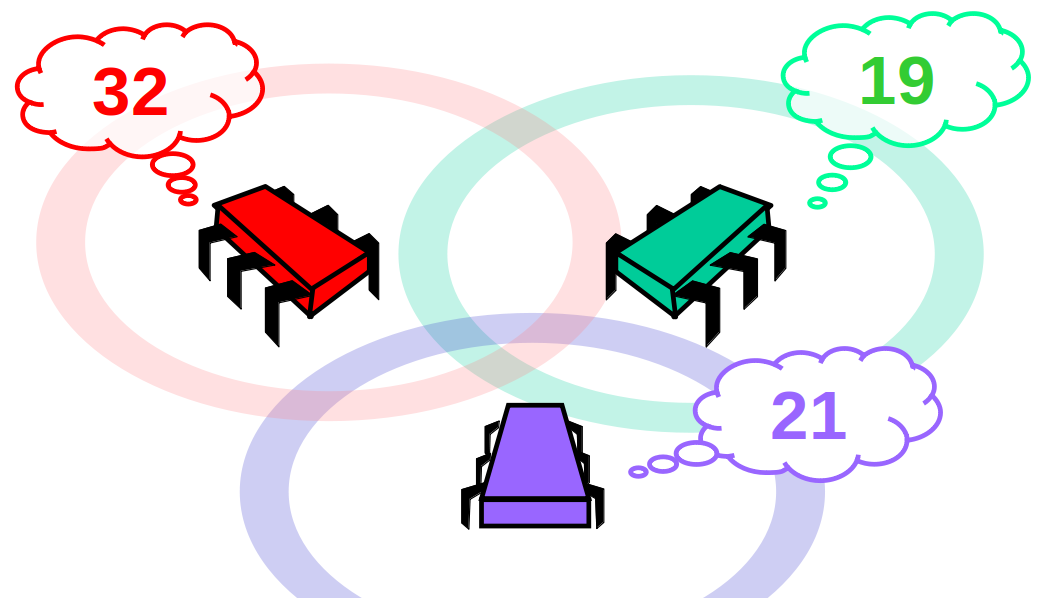
\includegraphics[width=0.5\textwidth]{./pics/consensus/cons1.png}
\end{center}
\end{frame}

\begin{frame}[noframenumbering]{They communicate}

\begin{center}
  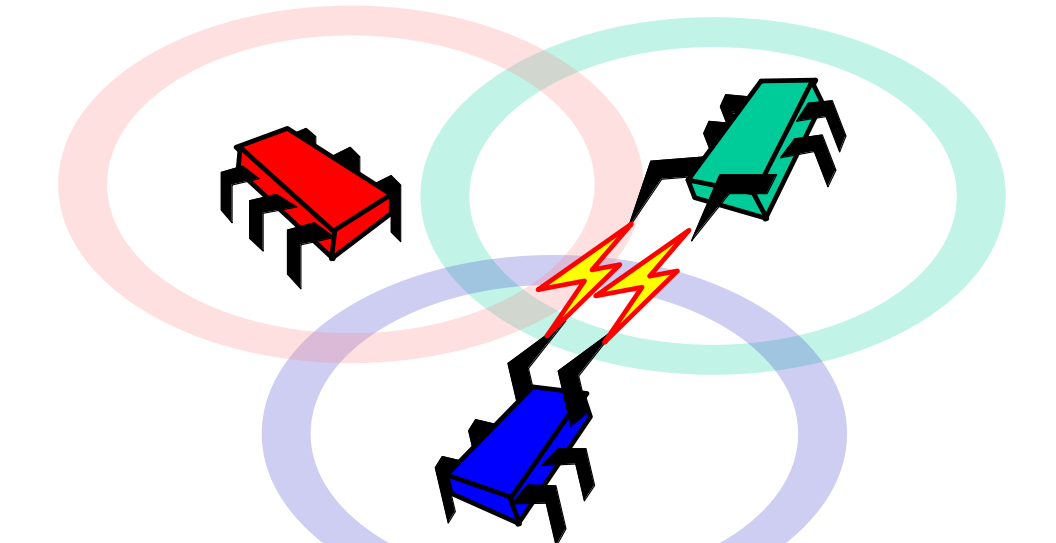
\includegraphics[width=0.5\textwidth]{./pics/consensus/cons2.png}
\end{center}

\end{frame}

\begin{frame}[noframenumbering]{They agree on some input}

\begin{center}
  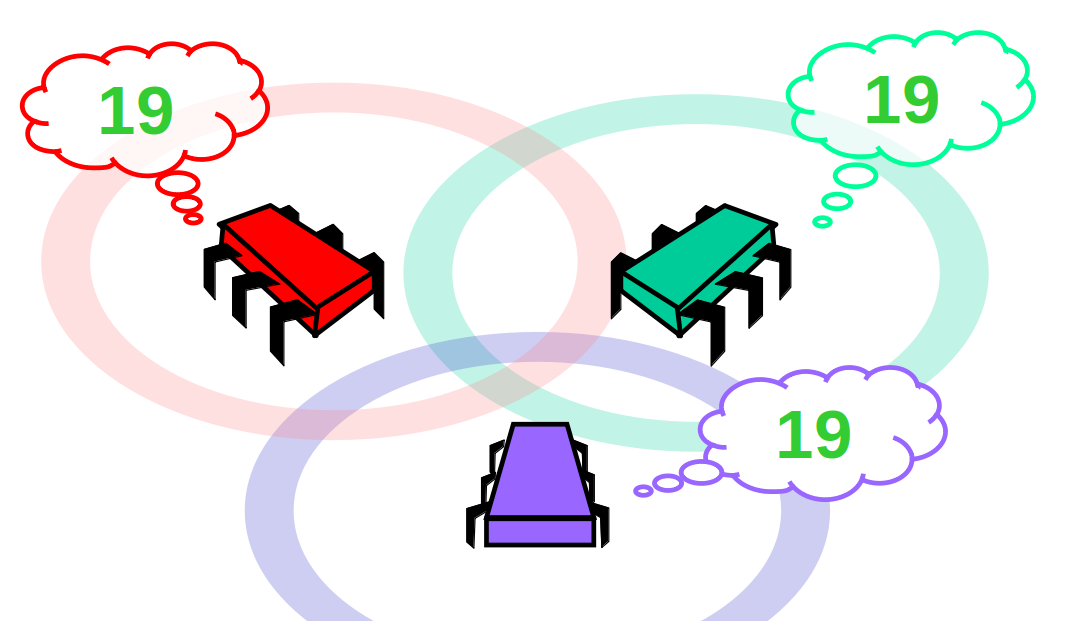
\includegraphics[width=0.5\textwidth]{./pics/consensus/cons3.png}
\end{center}
\end{frame}


\begin{frame}{Consensus}

\begin{itemize}
  \item \textbf{Consistent}: all threads decide the same value
  \item \textbf{Valid}: the common decision value is some thread's input
\end{itemize}

\pause

\begin{theorem}
  There is no wait-free implementation of n-thread consensus from read-write registers
\end{theorem}

\pause

Implication:
\begin{itemize}
  \item Asynchronous computability different from Turing computability
\end{itemize}

\pause

Read-write registers formalized in terms of safe/regular/atomic concurrent objects.

\pause

Theorem could be adapted to:

\begin{itemize}
  \item Registers
  \item Message-passing
  \item Carrier pigeons
  \item Any kind of asynchronous computation
\end{itemize}

\end{frame}

\begin{frame}{Consensus number}

An object \textbf{X} has \textit{consensus number} \textbf{n}
\begin{itemize}
  \item If it can be used to solve \textbf{n}-thread consensus
  \begin{itemize}
    \item Take any number of instances of \textbf{X} 
    \item together with atomic read/write registers
    \item and implement \textbf{n}-thread consensus
  \end{itemize}
  \item But not \textbf{(n+1)}-thread consensus
\end{itemize}

\pause

\begin{theorem}
  Atomic read/write registers have consensus number 1
\end{theorem}

Atomic registers cannot implement\only<3->{\textbf{ wait-free}} multiple assignment
\begin{itemize}
  \item Single write/multi read OK
  \item Multi write/multi read impossible
\end{itemize}

\end{frame}

\begin{frame}{Consensus numbers measure synchronization power}

\begin{theorem}
\begin{itemize}
  \item If you can implement \textbf{X} from \textbf{Y}
  \item And \textbf{X} has consensus number \textbf{c}
  \item Then \textbf{Y} has consensus number at least \textbf{c}
\end{itemize}
\end{theorem}

\pause

Registers have consensus number \textbf{1}

\pause

There are practically interesting problems that require higher consensus number

\pause

What should we do next?

\end{frame}

% \section{Q\&A}
% \begin{frame}{Q\&A session}
% 
% here are examples, are they linearizable
% 
% are they correct
% 
% again example of non-composable correct stuff that is not correct
% 
% which register is the best
% 
% why snapshot is not consensus
% 
% why temstamping snapshot is not consensus
% 
% Theory: filer lock solves N-thread coordination
% Theory: any N-thread coordination requires at lewast N atomic regs
% Theory: atomic reg consensus number is 1
% Contradiction?
% 
% \end{frame}

% \begin{frame}{You know too much}
% 
% A lot of information subtly connected with each other.
% 
% A lot of therory results, focused on "useful" definition (linearizability, wait-free)
% 
% Real life loves locks, it is ok to have even not obstruction-free algorithm and we have a lot of primitives (atomic registers of no use)
% 
% So know we will talk about more deep practical aspects (this lecture: some basixcs, and next lecture about h/w stuff)
% 
% And again: it will be a lot of subtly conected stuff. You are expected to have questions, do homework and ask help from TAs! 
% \end{frame}

\section{Read-Modify-Write}
\showTOC

\begin{frame}[fragile]{Read-Modify-Write Objects}

Method call
\begin{itemize}
  \item Returns previous value \textbf{x}
  \item Replaces \textbf{x} with \texttt{mumble(\textbf{x})}
\end{itemize}

\pause
\begin{minted}{java}
public abstract class RMWRegister {
  private int value;
  public int synchronized getAndMumble() {
    int prior  = value;
    value = mumble(value);
    return prior;
  }
}
\end{minted}

\pause

RMW everywhere!

\begin{itemize}
  \item Most synchronization instructions are RMW methods
  \item The rest can be trivially transformed into RMW methods
\end{itemize}

\end{frame}


\begin{frame}[t,fragile]{Read-Modify-Write: read}

\begin{minted}{java}
public abstract class RMWRegister {
  private int value;
  public int synchronized read() {
    int prior  = value;
    value = value; // mumble == identity
    return prior;
  }
}
\end{minted}

\end{frame}

\begin{frame}[t,fragile,noframenumbering]{Read-Modify-Write: getAndSet}

\begin{minted}{java}
public abstract class RMWRegister {
  private int value;
  public int synchronized getAndSet(int v) {
    int prior  = value;
    value = v; // mumble(x) = v, constant
    return prior;
  } 
}
\end{minted}

\end{frame}

\begin{frame}[t,fragile,noframenumbering]{Read-Modify-Write: getAndIncrement}

\begin{minted}{java}
public abstract class RMWRegister {
  private int value;
  public int synchronized getAndIncrement() {
    int prior  = value;
    value = value + 1; // mumble(x) = x + 1
    return prior;
  }
}
\end{minted}
\end{frame}

\begin{frame}[t,fragile,noframenumbering]{Read-Modify-Write: getAndAdd}

\begin{minted}{java}
public abstract class RMWRegister {
  private int value;
  public int synchronized getAndAdd(int a) {
    int prior  = value;
    value = value + a; // mumble(x) = x + a
    return prior;
  }
}
\end{minted}

\end{frame}

\begin{frame}[t,fragile,noframenumbering]{Read-Modify-Write: compareAndSet}

\begin{minted}{java}
public abstract class RMWRegister {
  private int value;
  public boolean synchronized compareAndSet(int expected, int update) {
    int prior = value;       // load witness value
    if (value == expected) { // if current value equals to expected
      value = update;        // then replace it with update
      return true;           // and return with success
    }
    return false;            // else return with failure, change nothing
  }
}
\end{minted}

\end{frame}

\begin{frame}[t,fragile,noframenumbering]{Read-Modify-Write: compareAndExchange}

\begin{minted}{java}
public abstract class RMWRegister {
  private int value;
  public int synchronized compareAndExchange(int expected, int update) {
    int prior = value;       // load witness value
    if (value == expected) { // if current value equals to expected
      value = update;        // then replace it with update      
    }
    return prior;            // return witness value
  }
}
\end{minted}
\end{frame}


\begin{frame}[fragile]{Read-Modify-Write: now you know it}

AtomicInteger\footnote{\tiny\url{https://docs.oracle.com/en/java/javase/11/docs/api/java.base/java/util/concurrent/atomic/AtomicInteger.html}}:
\pause
\begin{itemize}
  \item \texttt{get()}, \texttt{getAndSet(int)}
  \pause
  \item \texttt{incrementAndGet()}, \texttt{addAndGet(int)}
  \pause
  \item \texttt{compareAndSet(int,int)}, \texttt{compareAndExchange(int,int)}
  \pause
  \item \texttt{updateAndGet(java.util.function.IntUnaryOperator)}
  \item \texttt{accumulateAndGet(int,java.util.function.IntBinaryOperator)}  
\end{itemize}

\pause
Atomic*\footnote<6->{\tiny\url{https://docs.oracle.com/en/java/javase/11/docs/api/java.base/java/util/concurrent/atomic/package-summary.html}}

\begin{itemize}
  \item AtomicBoolean
  \item AtomicInteger, AtomicIntegerArray
  \item AtomicLong, AtomicLongArray
  \item AtomicReference, AtomicReferenceArray
  \pause
  \item AtomicMarkableReference, AtomicStampedReference
\end{itemize}

\end{frame}


\begin{frame}[fragile]{Atomic RMW: what's the point?}

General form of atomic RMW:
\begin{minted}{java}
public int synchronized getAndMumble() {
  int prior  = value;
  value = mumble(value);
  return prior;
}
\end{minted}

\pause
Interesting if and only if it is a non-blocking wait-free operation
\pause
\begin{itemize}
  \item Finishes in constant time
  \item Even in case of contention
  \item Independently of thread scheduling
  \pause
  \item Looks like a "mutex on steroids"
  \pause
  \item Supported on hardware level
\end{itemize}

\end{frame}


\begin{frame}[fragile,noframenumbering]{Atomic RMW: what's the point?}

\begin{minted}{java}
public int synchronized getAndMumble() {
  int prior  = value;
  value = mumble(value);
  return prior;
}
\end{minted}

Non-blocking wait-free operation
\begin{itemize}
  \item Finishes in constant time
  \item Even in case of contention
  \item Independently of thread scheduling
\end{itemize}

\pause

\begin{theorem}
Any non-trivial RMW object has consensus number at least 2
\end{theorem}

\pause

\begin{itemize}
  \item No wait-free implementation of RMW registers from atomic registers
  \item Hardware RMW instructions not just a convenience
\end{itemize}

\end{frame}


\begin{frame}[fragile]{Foundations: here we go again}

Atomic registers
\begin{itemize}
  \item From safe SRSW Boolean register \pause up to atomic MRMW Integer register \pause and atomic snapshot of $N$ registers
\end{itemize}
\pause
This journey required a lot of complicated wait-free constructions! \pause And in the very end ... 

\pause 

\begin{theorem}
  Atomic read/write registers have consensus number 1
\end{theorem}

\pause
Atomic RMW registers
\begin{itemize}
  \item Generalization of any "local" \ synchronized operation 
\end{itemize}
\pause Could implement a lot of even more complicated wait-free algorithms! \pause And in the very end ... 

\pause

\begin{theorem}
Any non-trivial RMW object has consensus number at least 2
\end{theorem}

\pause

When will we stop?

\end{frame}


\begin{frame}[fragile]{Consensus: final point}

\begin{theorem}
  Atomic read/write registers have consensus number 1
\end{theorem}

\begin{theorem}
Any non-trivial RMW object has consensus number at least 2
\end{theorem}

\pause

\begin{theorem}
 \texttt{getAndSet}, \texttt{getAndIncrement}, \texttt{getAndAdd} have consensus number exactly 2
\end{theorem}

\pause

\begin{theorem}
\texttt{compareAndSet} has $\infty$ consensus number
\end{theorem}

\end{frame}


\begin{frame}[fragile,noframenumbering]{Consensus: final point}
\begin{theorem}
\texttt{compareAndSet} has $\infty$ consensus number
\end{theorem}

\pause

\begin{minted}{java}
public class RMWConsensus {
  private AtomicInteger r = new AtomicInteger(-1); // init with -1
  private int[] proposed = new int[N]; // values proposed by threads
  public int decide(int value) { 
    int i = ThreadID.get();   // I am thread i
    proposed[i] = value;      // I propose value
    r.compareAndSet(-1, i);   // try to set my id as `winner`
    return proposed[r.get()]; // return value proposed by winner
  }
}
\end{minted}
\end{frame}


\begin{frame}[fragile]{The consensus hierarchy}

\begin{itemize}
  \item \textbf{1}. Read/Write Registers, Snapshots ...

  \item \textbf{2}. \texttt{getAndSet}, \texttt{getAndIncrement} ...

  \item ...

  \item $\infty$. \texttt{compareAndSet} ...
\end{itemize}

\pause

Multiprocessor concurrent environment is \textbf{very} friendly to wait-free algorithms. Hardware engineers know how to efficiently implement \texttt{compareAndSet}.
\pause We will discuss it in the very next Lecture~\cacheCoherencyNum \ (cache coherency).

\pause
Some other environments -- distributed systems, supercomputers, telegraph, pigeon posts etc. -- could be \textbf{different}. Now you know how to do the analysis of "computability" \ in such environments.

\pause
Challenges of the new era:
\begin{itemize}
  \item Highly distributed systems (internet nodes, geographically distributed data centers) with non-guaranteed message delivery (UDP)
  \item Heterogeneous computing (CPU, GPU, FPGA, GPGPU ...)
\end{itemize}

\end{frame}

\section{Concurrent Counter: puzzlers}
\showTOC

\begin{frame}[t,fragile]{SynchronizedCounter}

\begin{minted}{java}
public class SynchronizedCounter {
    private long cnt;
    public SynchronizedCounter(long initial) { this.cnt = initial; }
    // assume delta > 0
    public synchronized void increment(int delta) { cnt += delta; }
    public synchronized long get() { return cnt; }
}
\end{minted}

\begin{itemize}  
  \item Wait-free, Lock-free, Obstruction-free?
  \item Starvation-free, Deadlock-free?
\end{itemize}

\end{frame}

\begin{frame}[t,fragile,noframenumbering]{FairLockedCounter}

\begin{minted}{java}
public class FairLockedCounter {
    private long cnt;
    private final Lock lock = new ReentrantLock(/* fair = */ true); 
    public FairLockedCounter(long initial) { this.cnt = initial; }
    public void increment(int delta) { 
      lock.lock() try { cnt += delta; } finally { lock.unlock(); } 
    }
    public long get() { 
      lock.lock(); try { return cnt; } finally { lock.unlock(); }
    }
}
\end{minted}

\begin{itemize}  
  \item Wait-free, Lock-free, Obstruction-free?
  \item Starvation-free, Deadlock-free?
\end{itemize}

\end{frame}


\begin{frame}[t,fragile]{AtomicLoopCounter}

\begin{minted}{java}
public class AtomicLoopCounter {
    private long cnt;
    private final AtomicBoolean status = new AtomicBoolean(false); 
    public AtomicLoopCounter(long initial) { this.cnt = initial; }
    public void increment(int delta) { 
      while (status.getAndSet(true) == true) {}
      try { cnt += delta; } finally { status.set(false); }
    }
    public long get() { 
      while (status.getAndSet(true) == true) {}
      try { return cnt; } finally { status.set(false); }
    }}
\end{minted}

\begin{itemize}  
  \item Wait-free, Lock-free, Obstruction-free?
  \item Starvation-free, Deadlock-free?
\end{itemize}

\end{frame}

\begin{frame}[t,fragile]{AtomicIncCounter}

\begin{minted}{java}
public class AtomicIncCounter {
    private final AtomicLong cnt = new AtomicLong(0); 
    public AtomicIncCounter(long initial) { cnt.set(initial); }
    public void increment(int delta) { 
      cnt.getAndAdd(delta);
    }
    public long get() { 
      return cnt.get();
    }}
\end{minted}

\begin{itemize}  
  \item Wait-free, Lock-free, Obstruction-free?
  \item Starvation-free, Deadlock-free?
\end{itemize}

\end{frame}


\begin{frame}[t,fragile]{AtomicCASCounter}

\begin{minted}{java}
public class AtomicCASCounter {
    private final AtomicLong cnt = new AtomicLong(0); 
    public AtomicCASCounter(long initial) { cnt.set(initial); }
    public void increment(int delta) {
      long expected = cnt.get();
      while (true) {        
        long witness = cnt.compareAndExchange(expected, expected + delta);
        if (witness == expected) { return; } else { expected = witness; }        
      }
    }
    public long get() { return cnt.get(); }}
\end{minted}

\begin{itemize}  
  \item Wait-free, Lock-free, Obstruction-free?
  \item Starvation-free, Deadlock-free?
\end{itemize}

\end{frame}


\begin{frame}[t,fragile]{ReplicatedCounter}

\begin{minted}{java}
static final ThreadLocal<Long> privateCounter = new ThreadLocal<Long>();
public void increment(int delta) {
  privateCounter.set(privateCounter.get() + delta);   
}
public long get() { 
  long result = 0;
  for (Thread t: ALL_THREADS) result += t.privateCounter.get(); // PSEUDOCODE
  return result;
}
\end{minted}


\begin{itemize}  
  \item Wait-free, Lock-free, Obstruction-free?
  \item Starvation-free, Deadlock-free?
  \pause
  \item Linearizable? \pause What if \texttt{ThreadLocal} are Atomic MRMW registers?
\end{itemize}
\end{frame}


\begin{frame}[t,fragile]{Concurrent counters: summary}

\begin{itemize}  
  \item Progress conditions describe the whole method/algorithm/object
  \pause
  \item Fixed number lines of code -- does not mean wait-free
  \pause
  \item No explicit locks -- does not mean lock-free
  \pause
  \item \texttt{synchronized} does not guarantee starvation freedom
  \pause
  \item \texttt{ReentrantLock} could be configured as fair (starvation-free)
  \pause
  \item \texttt{CAS} is not always better than \texttt{getAndAdd}
  \pause
  \item Wait-free and smart does not mean correct (consistent or linearizable)
\end{itemize}

\end{frame}

\section{Basic spin locks}
\showTOC

\begin{frame}[fragile]{Test-And-Set: non-reentrant boolean spin lock}

\begin{minted}{java}
class TASlock {
  private static final boolean LOCKED = true, UNLOCKED = false;
  private final AtomicBoolean state = new AtomicBoolean(UNLOCKED);
  void lock() {
    while (true) {
      boolean before = state.getAndSet(LOCKED); // <-----------|
      if (before == UNLOCKED) { return; } // I win             |
      else {}                             // I lose, repeat ---+      
  }}
  void unlock() { state.set(UNLOCKED); }
}
\end{minted}

\pause
\begin{itemize}
  \item Pros: easy to implement, easy to prove correctness, ultra-fast ownership handoff
  \item Cons: burn CPU, contention on memory bus
\end{itemize}
\end{frame}


\begin{frame}{Test-And-Set: reentrant spin lock}
\begin{homeworkmail}{Task~\taskReentrantTAS}{
    Replace \texttt{AtomicBoolean} with \texttt{AtomicReference(Thread.cuurentThread)} and make TAS lock reentrant. Provide at least 3 tests written in JCStress.
}
\end{homeworkmail}
\end{frame}


\begin{frame}[fragile]{Test-And-Set: non-reentrant boolean spin lock}

\begin{minted}{java}
class TASlock {
  private static final boolean LOCKED = true, UNLOCKED = false;
  private final AtomicBoolean state = new AtomicBoolean(UNLOCKED);
  void lock() {
    while (true) {
      boolean before = state.getAndSet(LOCKED); // <-----------|
      if (before == UNLOCKED) { return; } // I win             |
      else {}                             // I lose, repeat ---+      
  }}
  void unlock() { state.set(UNLOCKED); }
}
\end{minted}

\begin{itemize}
  \item Pros: easy to implement, easy to prove correctness, ultra-fast ownership handoff.
  \item Cons: burn CPU, \textbf{contention on memory bus}. \only<2->{\textbf{WHAT?}}
\end{itemize}
\end{frame}

\begin{frame}{Memory bus}

\only<1>{
\begin{center}
  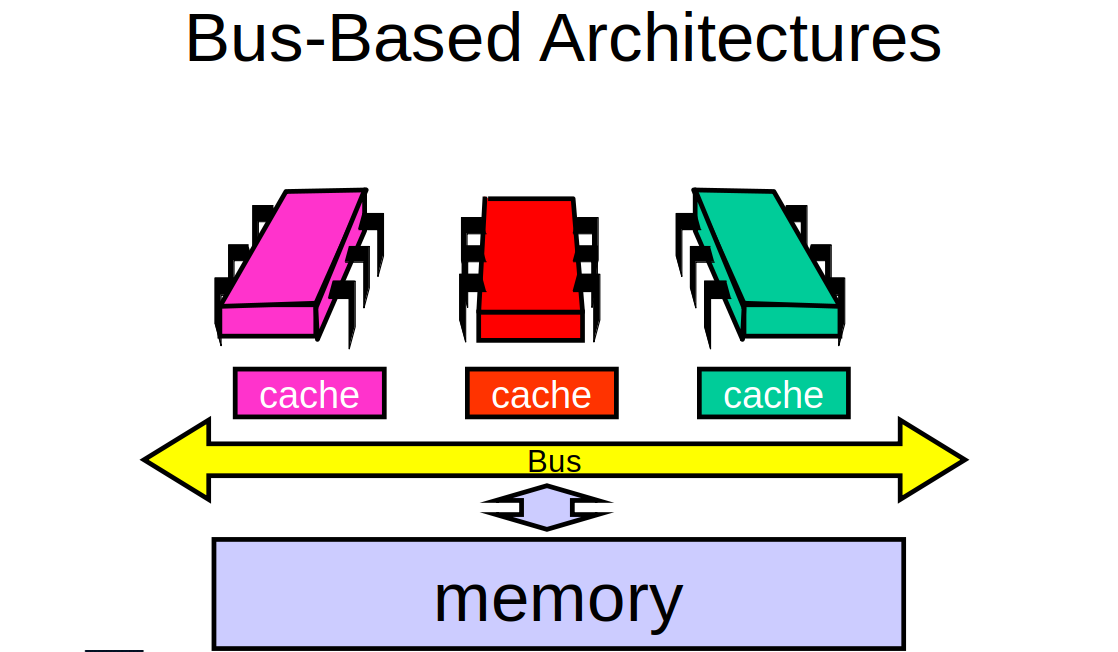
\includegraphics[width=0.5\textwidth]{./pics/cache/38.png}
\end{center}
}

\only<2>{
\begin{center}
  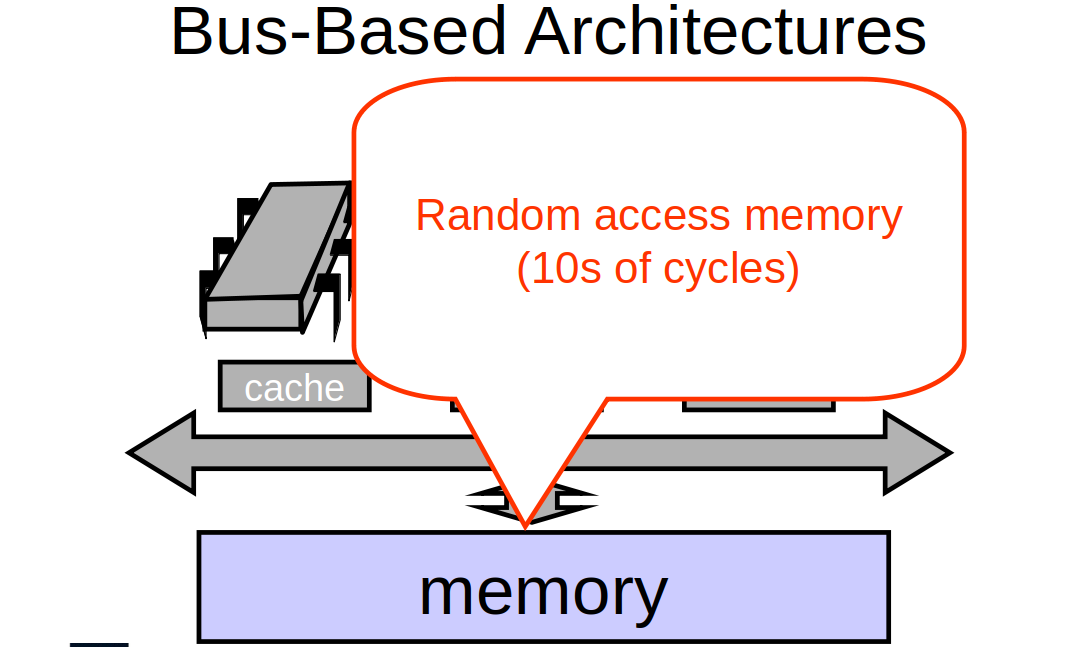
\includegraphics[width=0.5\textwidth]{./pics/cache/39.png}
\end{center}
}

\only<3>{
\begin{center}
  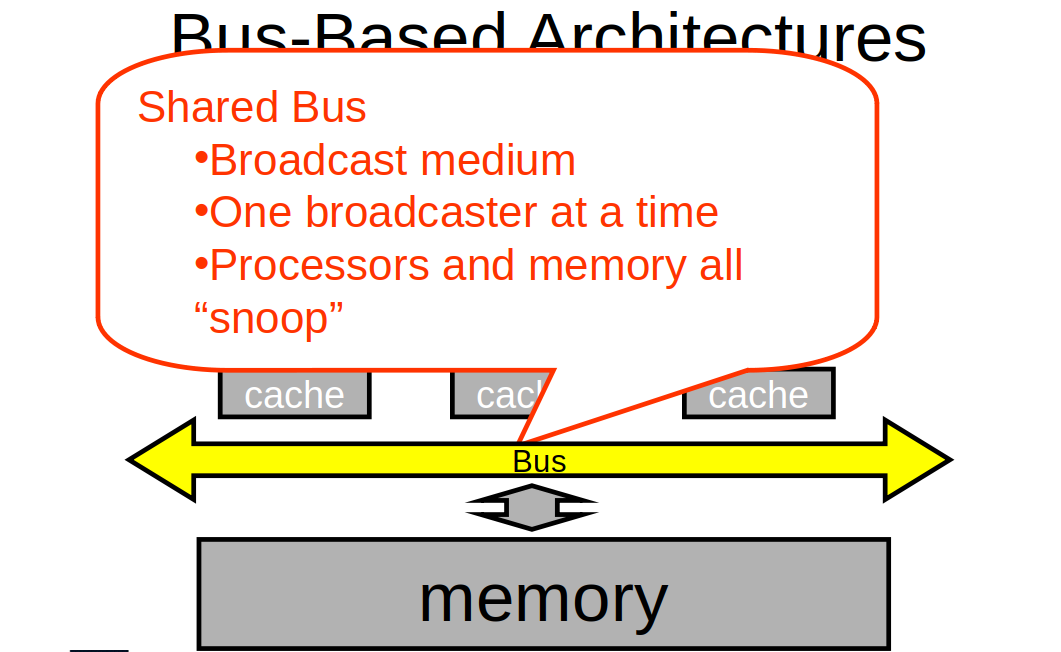
\includegraphics[width=0.5\textwidth]{./pics/cache/40.png}
\end{center}
}

\only<4>{
\begin{center}
  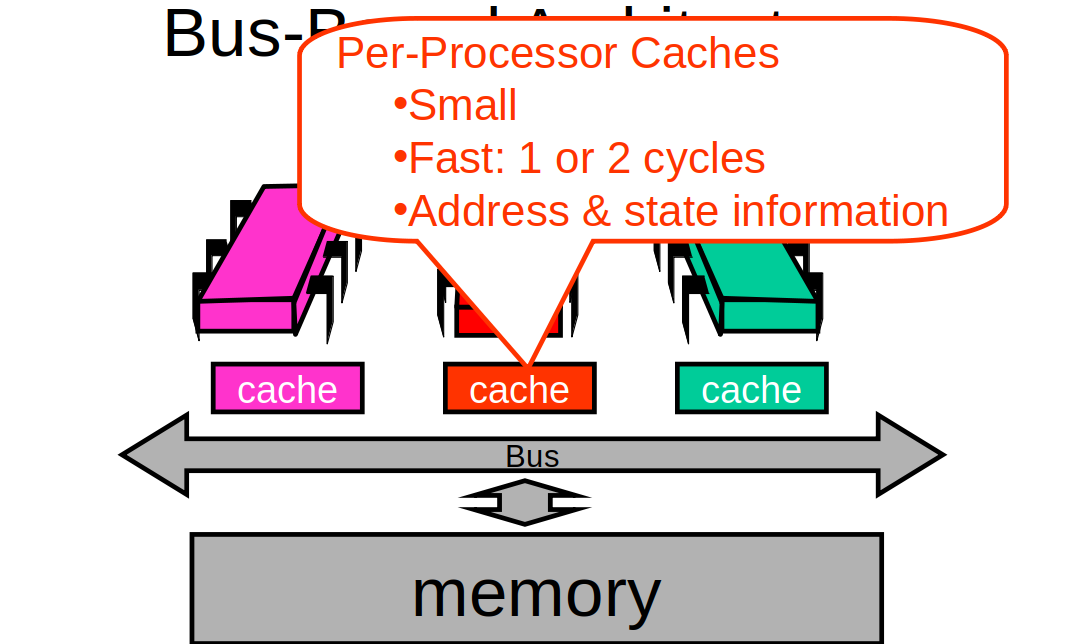
\includegraphics[width=0.5\textwidth]{./pics/cache/41.png}
\end{center}
}

\end{frame}

\begin{frame}{Cache}

\begin{itemize}
  \item \textbf{Cache hit} -- data found in local cache of current processor
  \item \textbf{Cache miss} -- up-to-date data must be found elsewhere
\end{itemize}

\pause

There are many questions related to cache-based design:
\begin{itemize}
  \item How many level of caches should be used?
  \item What is optimal size for each level?
  \item How to properly synchronize caches?
  \item How to move out stale data from cache?
  \item ... 
\end{itemize}

\pause

We will go deeper in next Lecture.

\pause

Today we will try to illustrate that even basic low-level knowledge helps to speed-up concurrent algorithms.

\end{frame}


\begin{frame}{Read data}

\only<1>{ \begin{center} 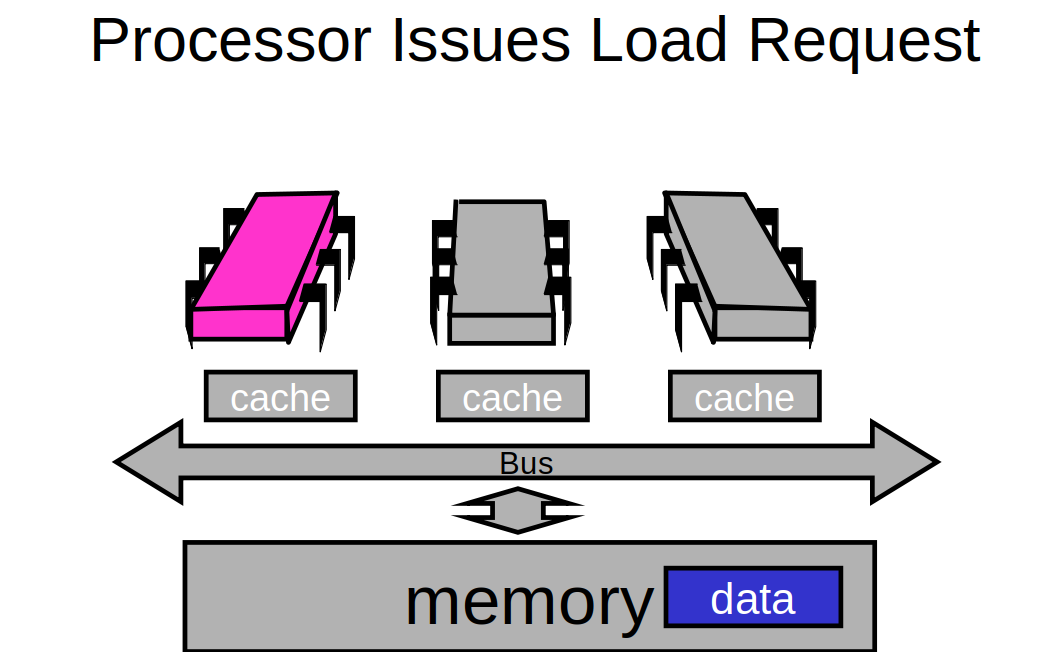
\includegraphics[width=0.5\textwidth]{./pics/cache/45.png} \end{center} }
\only<2>{ \begin{center} 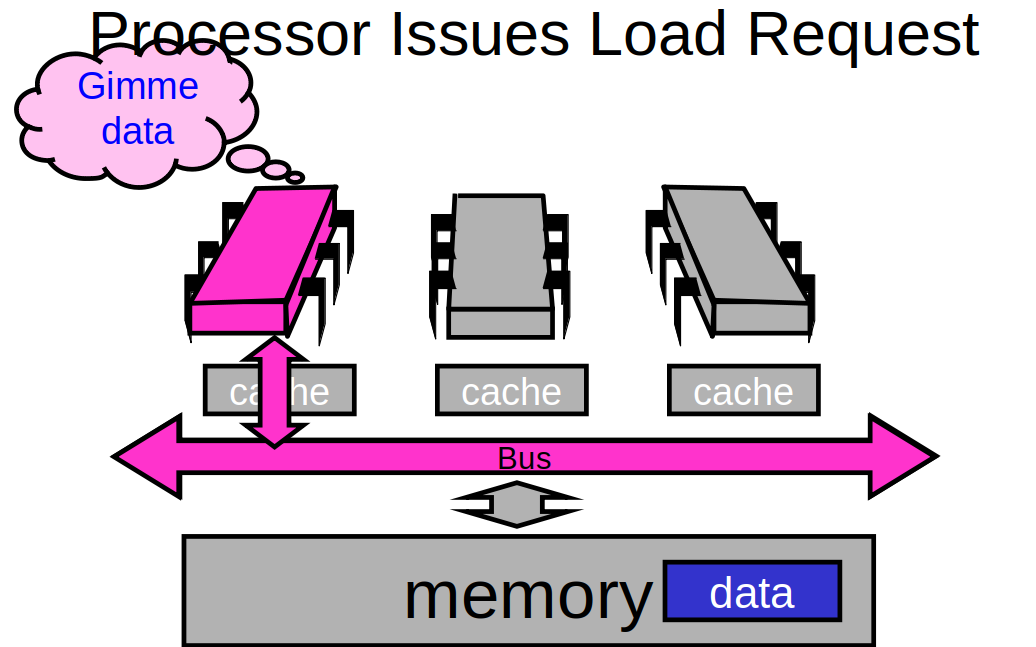
\includegraphics[width=0.5\textwidth]{./pics/cache/46.png} \end{center} }
\only<3>{ \begin{center} 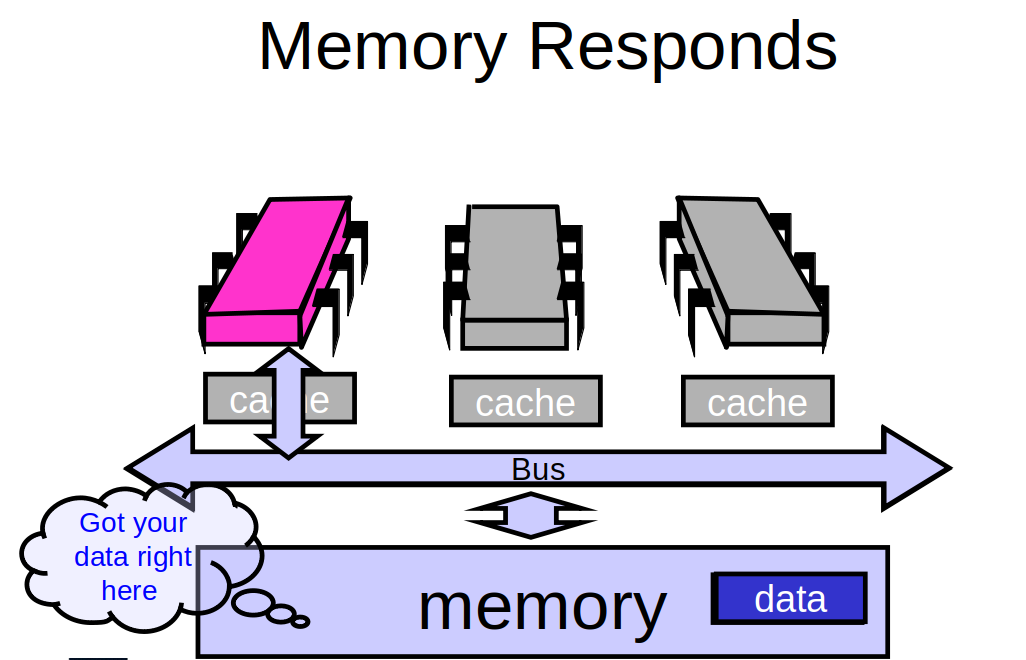
\includegraphics[width=0.5\textwidth]{./pics/cache/47.png} \end{center} }
\only<4>{ \begin{center} 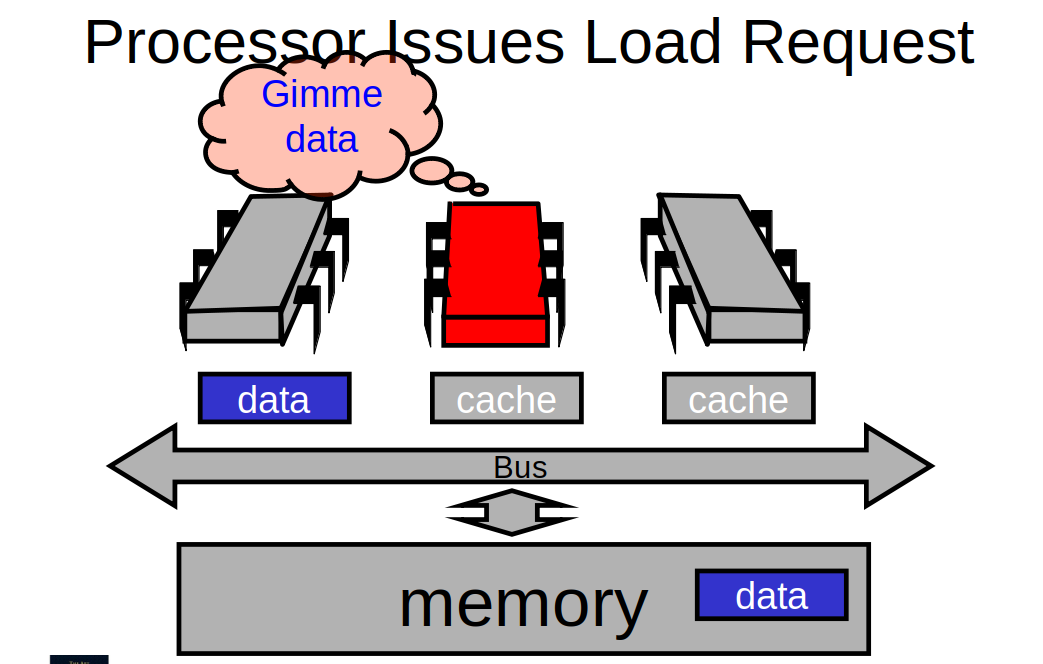
\includegraphics[width=0.5\textwidth]{./pics/cache/48.png} \end{center} }
\only<5>{ \begin{center} 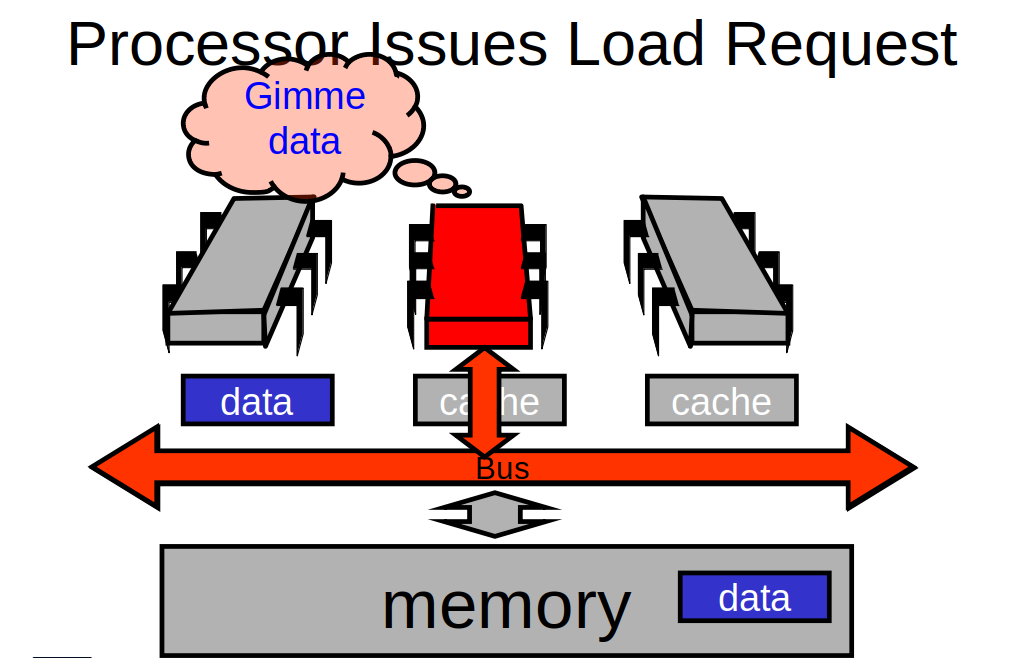
\includegraphics[width=0.5\textwidth]{./pics/cache/49.png} \end{center} }
\only<6>{ \begin{center} 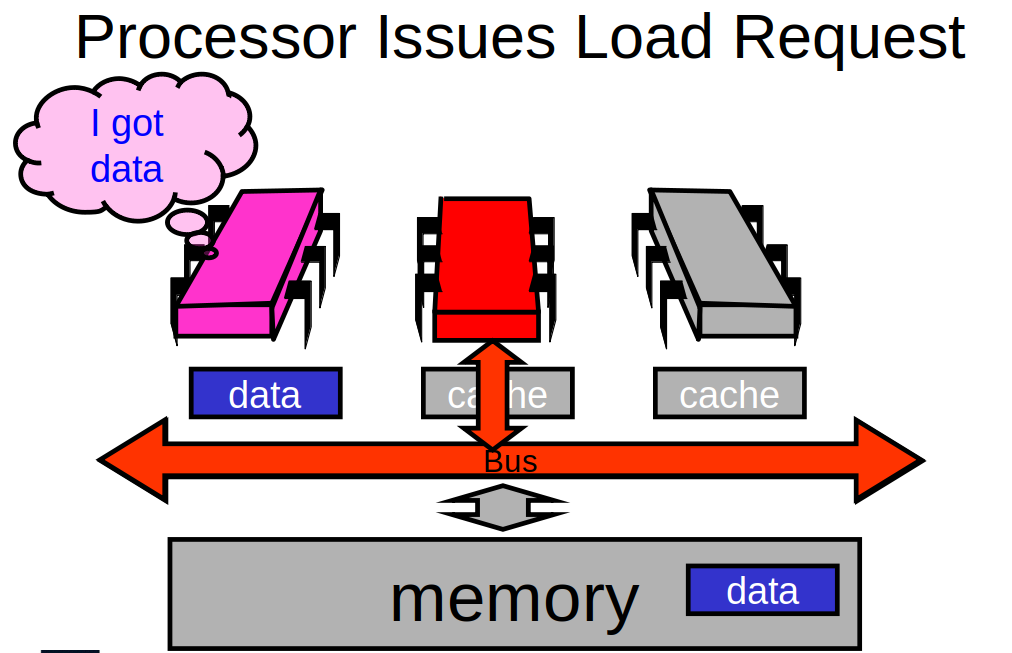
\includegraphics[width=0.5\textwidth]{./pics/cache/50.png} \end{center} }
\only<7>{ \begin{center} 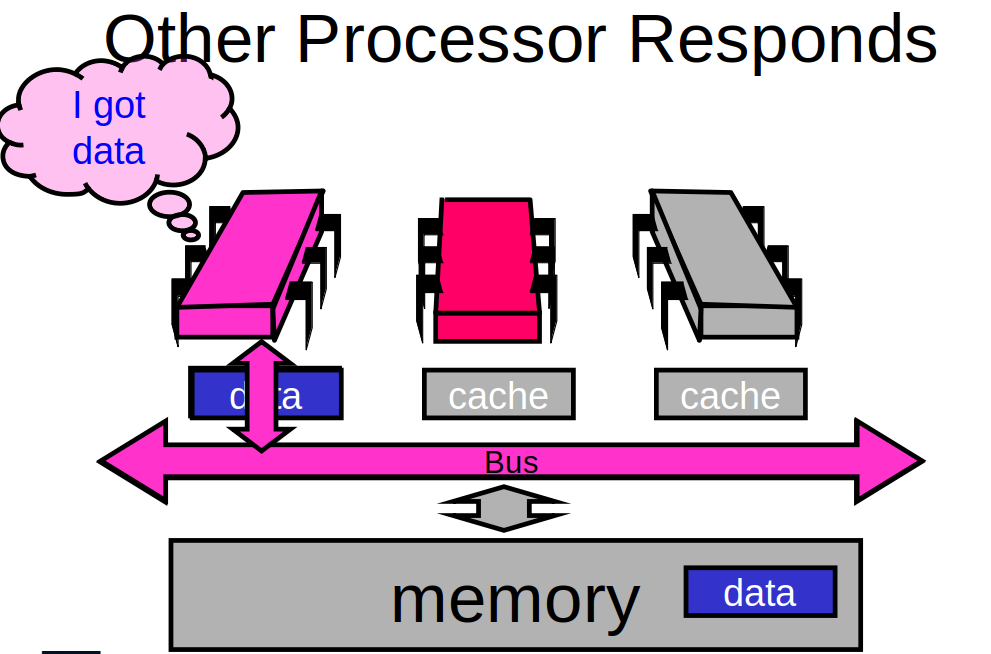
\includegraphics[width=0.5\textwidth]{./pics/cache/51.png} \end{center} }
\only<8->{ \begin{center} 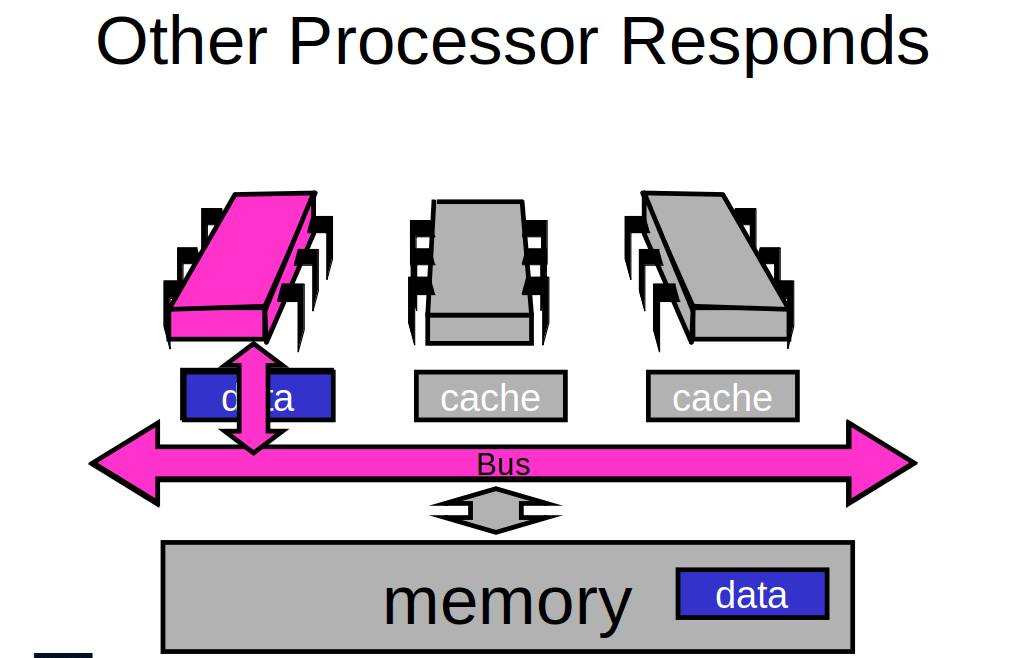
\includegraphics[width=0.5\textwidth]{./pics/cache/52.png} \end{center} }
\only<9->{
\begin{center}
  And now we have several copies of the same data in different places
\end{center}
}

\end{frame}

\begin{frame}{Modify data}

\only<1>{ \begin{center} 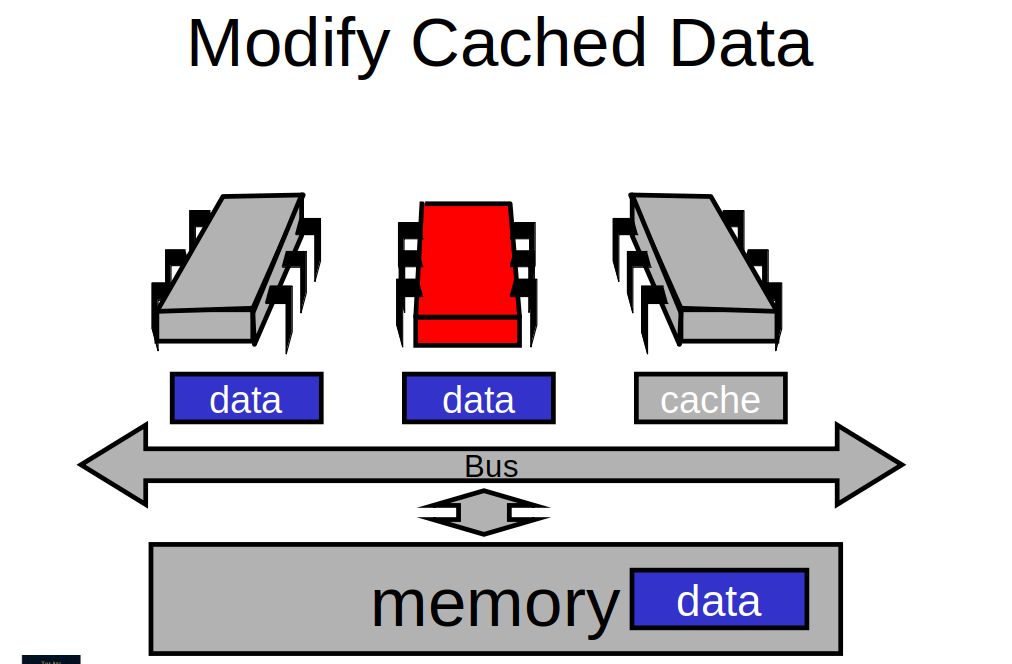
\includegraphics[width=0.5\textwidth]{./pics/cache/53.png} \end{center} }
\only<2>{ \begin{center} 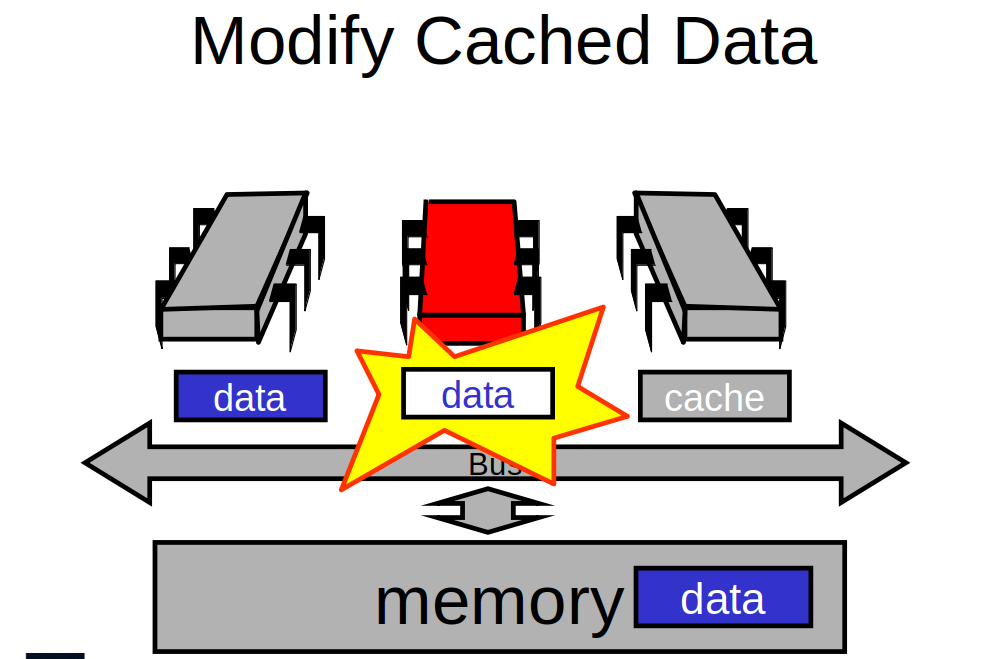
\includegraphics[width=0.5\textwidth]{./pics/cache/54.png} \end{center} }
\only<3>{ \begin{center} 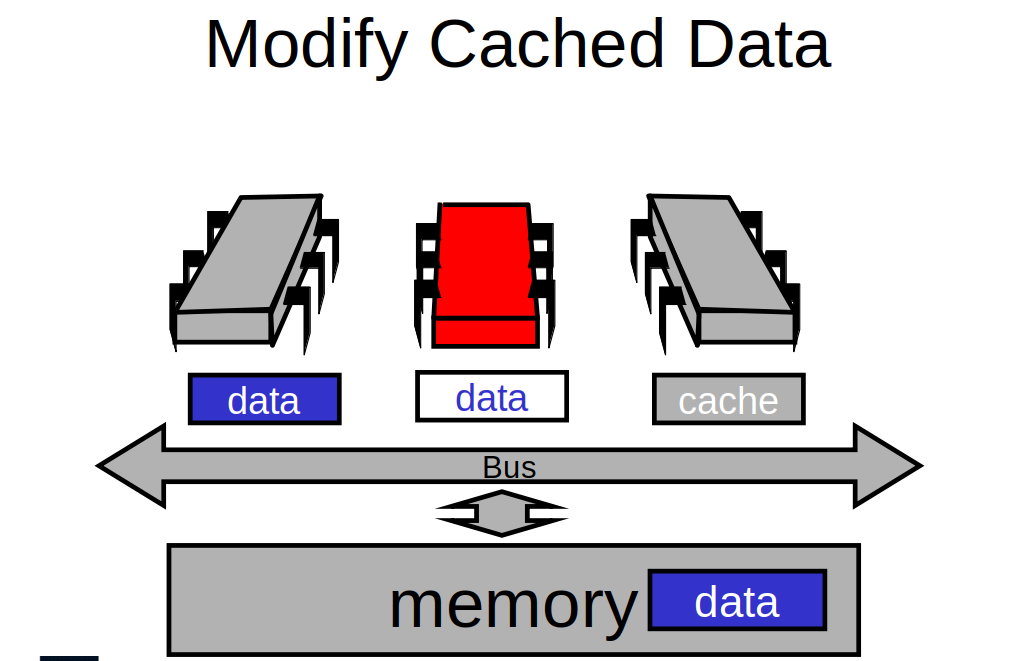
\includegraphics[width=0.5\textwidth]{./pics/cache/55.png} \end{center} }
\only<4>{ \begin{center} 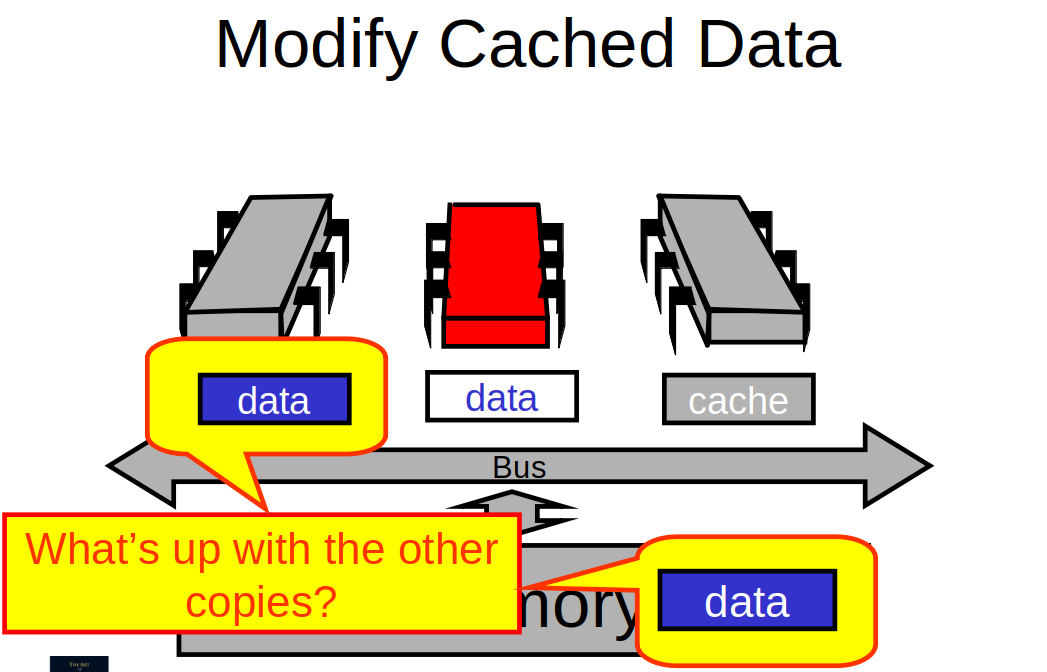
\includegraphics[width=0.5\textwidth]{./pics/cache/56.png} \end{center} }

\end{frame}


\begin{frame}{Cache coherence}

We have lots of copies of data
\begin{itemize}
  \item Original copy in memory 
  \item Cached copies at processors
\end{itemize}

\pause

Some processor modifies its own copy
\begin{itemize}
  \item What do we do with the others?
  \item How to avoid confusion?
\end{itemize}

\pause

Cache coherence protocol -- algorithm that handles such problems.

\pause

Low-level concurrent algorithm that is implemented in hardware
\begin{itemize}
  \pause
  \item No ReentrantLocks, Semaphores, ReadWriteLocks
  \item Critical for speed of the whole system (hope it is non-blocking)
  \pause
  \item Provides some consistency guarantees on "our view of" \ memory cells
\end{itemize}
\pause

What a joy that you have already encountered such tasks before!

\pause

Next Lecture will be s-o-o-o interesting.

\pause

Let's go back to the naive multiprocessor model.

\end{frame}

\begin{frame}{Cache coherence: invalidation}

We have lots of copies of data
\begin{itemize}
  \item Original copy in memory 
  \item Cached copies at processors
\end{itemize}

Some processor modifies its own copy

\pause
\begin{itemize}
  \item Broadcast a special message "invalidate data"
  \pause
  \item Ensure other processors replied to this as "Yes, sir!"
  \pause
  \item Now current processor is the unique owner of data, others will consult with him
  \pause
  \item Modify data
\end{itemize}
\end{frame}


\begin{frame}{Cache coherence: message passing}
Messages
\begin{itemize}
  \item Request for read, Respond with data
  \item Request for invalidate, Acknowledge invalidation
  \item Write-back modified data to main memory
\end{itemize}

\pause

Nanoseconds\footnote<2->{\tiny\url{https://americanhistory.si.edu/collections/object/nmah_692464}}:
\begin{center} 
  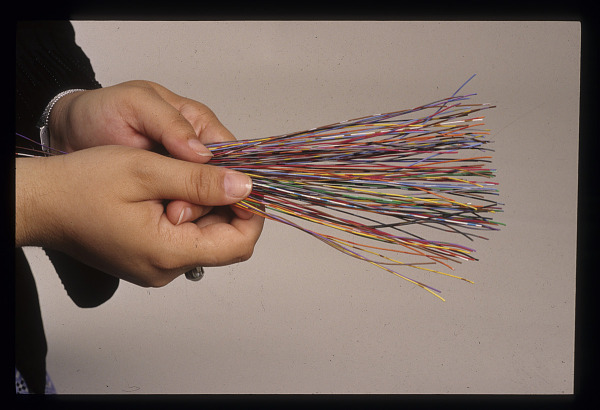
\includegraphics[width=0.4\textwidth]{./pics/nano.jpg} 
\end{center}
\end{frame}

\begin{frame}{Memory bus, cache coherence, multiprocessor: takeaways}

Multiprocessor systems have complicated memory subsystem
\begin{itemize}
  \pause
  \item Set of caches
  \pause
  \item synchronized with each other on low hardware level
  \pause
  \item using replication pattern (copy to read, invalidate for write)
  \pause
  \item to guarantee cache coherence (consistency of memory cell view)
\end{itemize}

\pause
Simplified cost model:
\begin{itemize}
  \item Read from private non-shared data is ultra-fast
  \item Write to private non-shared data is ultra-fast
  \item Read from private shared data is ultra-fast
  \item Write to shared data requires communication (invalidate and await)
  \item Read/write of non-cached location takes significant time
\end{itemize}

\end{frame}

\begin{frame}[fragile]{TASLock: reminder}

\begin{minted}{java}
class TASlock {
  private static final boolean LOCKED = true, UNLOCKED = false;
  private final AtomicBoolean state = new AtomicBoolean(UNLOCKED);
  void lock() {
    while (true) {
      boolean before = state.getAndSet(LOCKED); // <-----------|
      if (before == UNLOCKED) { return; } // I win             |
      else {}                             // I lose, repeat ---+      
  }}
  void unlock() { state.set(UNLOCKED); }
}
\end{minted}

\begin{itemize}
  \item Pros: easy to implement, easy to prove correctness, ultra-fast ownership handoff.
  \item Cons: burn CPU, \textbf{contention on memory bus}.
\end{itemize}
\end{frame}


\begin{frame}[fragile]{Test-and-Test-and-Set: non-reentrant boolean spin lock}

\begin{minted}{java}
class TATASlock {
  private static final boolean LOCKED = true, UNLOCKED = false;
  private final AtomicBoolean state = new AtomicBoolean(UNLOCKED);
  void lock() {
    while (true) {
      while (state.get() == LOCKED) {} // do not write if mutex is busy 
      if (state.getAndSet(LOCKED) == UNLOCKED) { // try acquire
        return;
}}}}
\end{minted}

\pause
Lock acquisition is OK, no excessive cache coherence bus traffic.

\pause
What happens on release?

\pause
Invalidation storm.

\end{frame}


\begin{frame}{Invalidation storm}

\only<1>{ \begin{center} 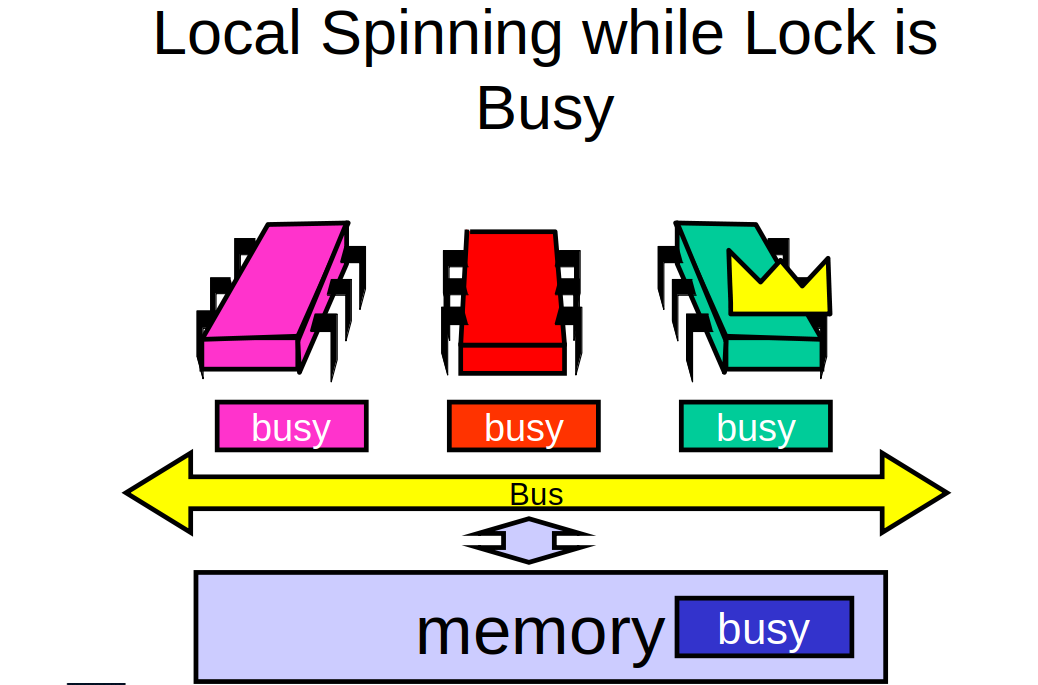
\includegraphics[width=0.5\textwidth]{./pics/storm/72.png} \end{center} }
\only<2>{ \begin{center} 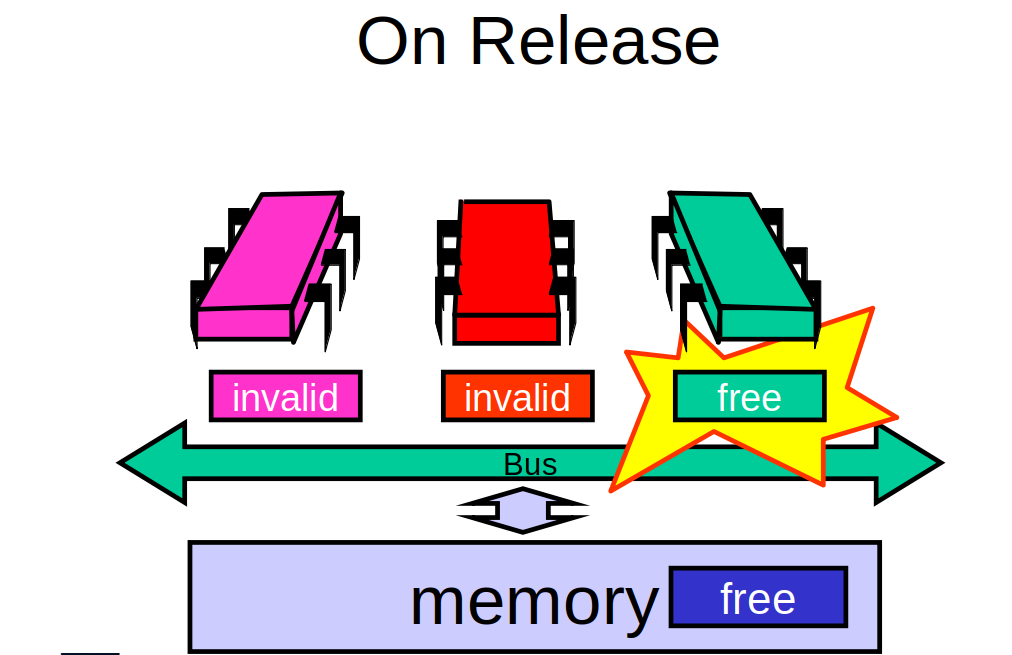
\includegraphics[width=0.5\textwidth]{./pics/storm/73.png} \end{center} }
\only<3>{ \begin{center} 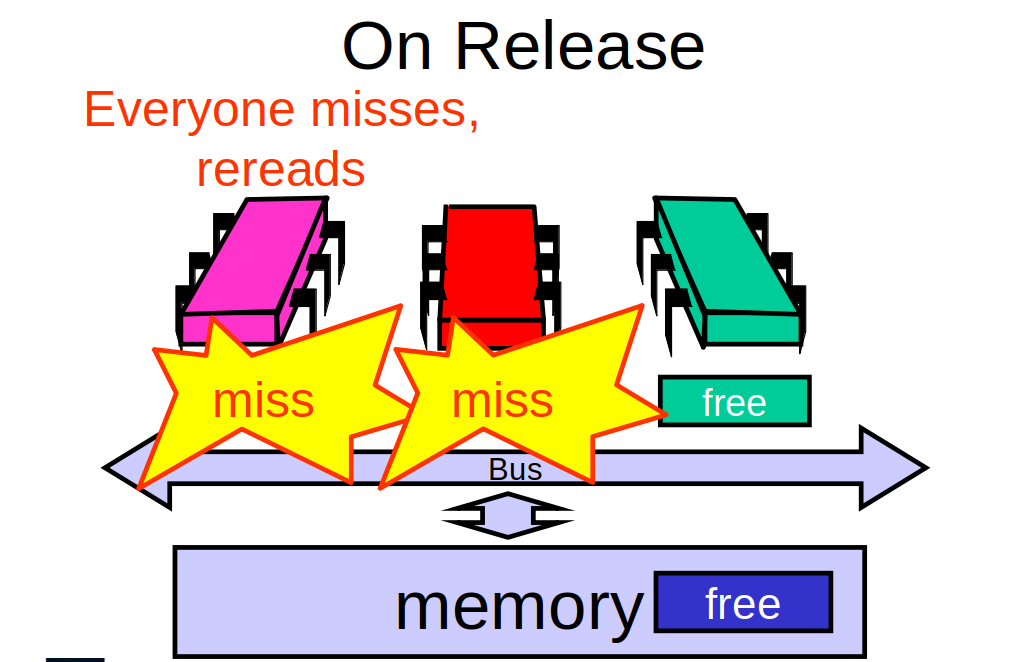
\includegraphics[width=0.5\textwidth]{./pics/storm/74.png} \end{center} }
\only<4>{ \begin{center} 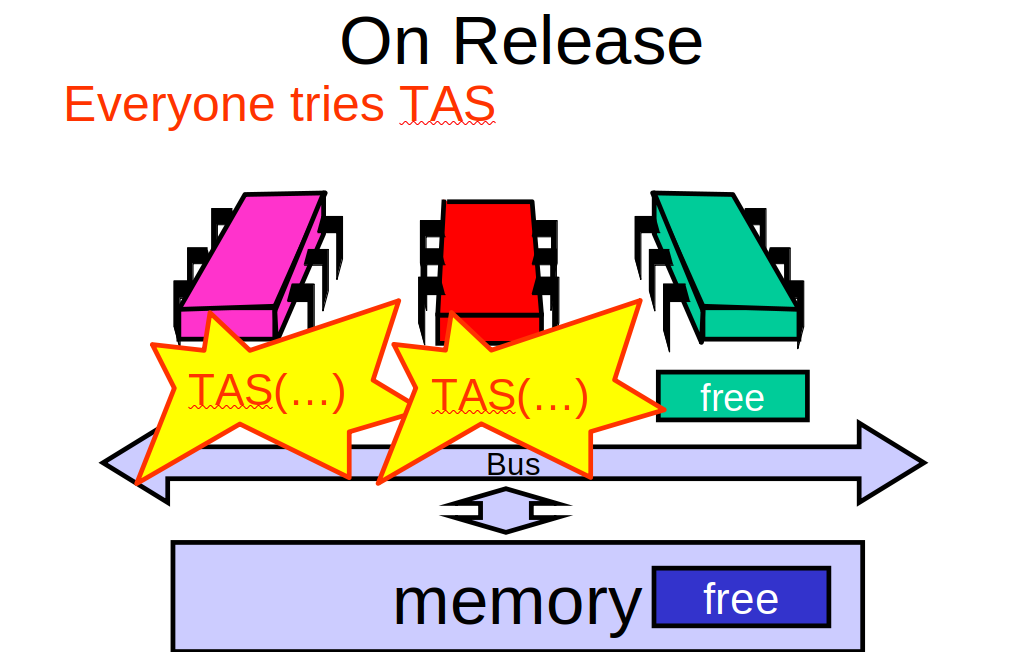
\includegraphics[width=0.5\textwidth]{./pics/storm/75.png} \end{center} }

\end{frame}


\begin{frame}[fragile]{TATAS: invalidation storm}

\begin{itemize}
  \item Everyone misses
  \pause
  \item Everyone does TAS
  \pause
  \item Invalidates others’ caches
  \pause
  \item Eventually \textit{quiesces} after lock acquired
\end{itemize}

\pause
How long does this take?  

\pause

General pattern for TATAS:
\begin{itemize}  
  \pause
  \item Acquire lock
  \pause
  \item Pause without using bus
  \pause
  \item Use bus heavily
\end{itemize}

\pause
\begin{itemize}  
  \item If pause > quiescence time
  \begin{itemize}
    \item critical section duration independent of number of threads
  \end{itemize}

  \pause
  \item If pause < quiescence time
  \begin{itemize}
    \item critical section duration slower with more threads
  \end{itemize}
\end{itemize}

\end{frame}

\begin{frame}[fragile]{Quiescence Time}

\only<1>{ \begin{center} 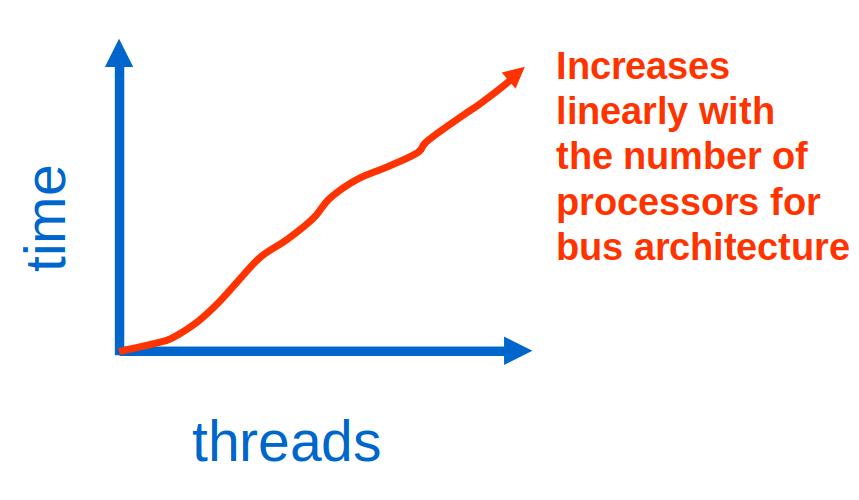
\includegraphics[width=0.7\textwidth]{./pics/storm/78.png} \end{center} }

\end{frame}


\begin{frame}[fragile]{Spin locks and hardware, you know so far}

\begin{itemize}
  \item Easy to implement and prove correctness
  \item Burn CPU for better responsiveness
  \item Read before trying to acquire lock, writes to actually shared memory are expensive
  \item Suffer from invalidation storm in contended environment when lock is released
\end{itemize}

\pause

Problems arise when
\begin{itemize}
  \pause
  \item Many threads compete for the single lock
  \pause
  \item Critical section is quite small ($\approx$ quiescence time of h/w)
  \pause
  \item Maybe application is misdesigned?
\end{itemize}

\pause

Any kind of "storm" \ (trap storm, invalidation storm, scheduler storm etc.) is a strong sign of misdesign. \pause
You could workaround it to some extent, but it will manifest itself later (more threads, faster h/w, better OS).

\pause
Anyway, let's try to avoid the invalidation storm and (maybe) improve our skills with "designing it right"

\end{frame}


% \begin{frame}{Cache contention/false sharing}
% 
% because you do not control allocation and we have caheline size 64-128 bytes
% 
% TODO: be covered in Lec-TODO of course
% 
% but in practice you need paddings @Contended and stuff
% \end{frame}


\begin{frame}[fragile]{Exponential Backoff}

\begin{minted}{java}
public void lock() {
  int delay = MIN_DELAY;
  while (true) {
    while (state.get() == LOCKED) {} // read-only polling
    if (lock.getAndSet(LOCKED) == UNLOCKED) return; // return on success
    sleep(random() % delay); // delay next write request on failure
    delay = Math.min(delay * 2, MAX_DELAY); // keep delay within bounds    
  }
}
\end{minted}

\pause
\begin{itemize}
  \item Trade-off: CPU overuse vs. latency
  \pause
  \item Still very naive, we will continue in Lecture~\advancedConcurrencyNum \ (queue locks)
\end{itemize}
\end{frame}


\begin{frame}[t,fragile]{Spin locks: summary}


\begin{itemize}
  \item Easy to implement and prove correctness
  \item Burn CPU vs. better responsiveness
  \item Actual performance depend on h/w (cache coherency) and application (contention)
\end{itemize}

\pause

\begin{center} 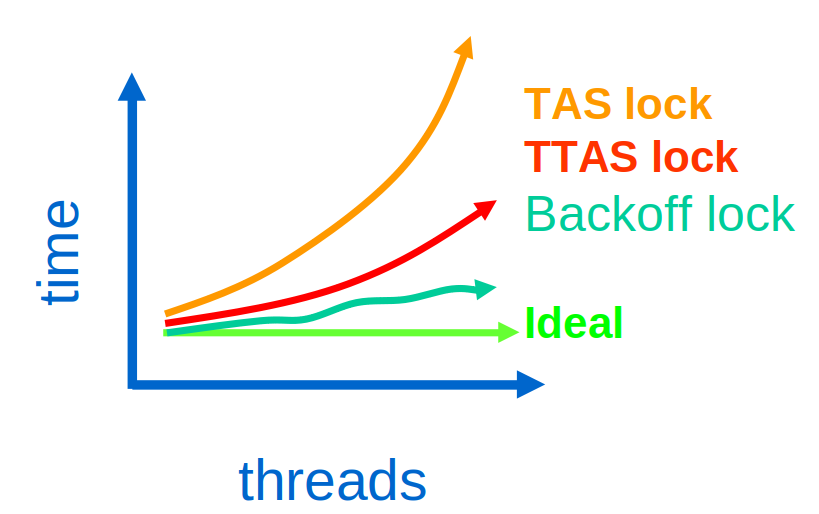
\includegraphics[width=0.5\textwidth]{./pics/locks.png} 
\end{center} 

\end{frame}


\begin{frame}[t,fragile,noframenumbering]{Spin locks: summary}

\begin{itemize}
  \item Easy to implement and prove correctness
  \item Burn CPU vs. better responsiveness
  \item Actual performance depend on h/w (cache coherency) and application (contention)
\end{itemize}

\textbf{Critically important}:
\begin{itemize}
  \pause
  \item Spin locking is a design pattern, building block for "normal" \ locking algorithms
  \pause
  \item \textbf{NEVER} use plain spin locks anywhere in production system\footnote<3->{\tiny\url{https://www.realworldtech.com/forum/?threadid=189711&curpostid=189723}} \pause unless you know what you are doing. \pause After finishing this introductory course on concurrency, you definitely \textbf{don't}.
\end{itemize}


\end{frame}



\begin{frame}{Spin locks: homework}

\begin{homeworkmail}{Task~\taskSpinMeasure}{
    Measure performance of \texttt{TASLock}, \texttt{TATASLock}, \texttt{ExpBackoffLock} on
    \begin{itemize}
      \item 1, 2, 3, 4, 5, 6, 7, 8, 16, 32 concurrent threads
      \item With small critical section (increment)
      \item With moderate critical section (compute n-th fibonacci number recursively)
    \end{itemize}
    using JMH or JCStress, plot resulting figures (with error bars!), explain gathered data.
}
\end{homeworkmail}
\end{frame}

\section{Lock-free stack and ABA}
\showTOC

\begin{frame}{Lock-free stack}

\begin{itemize}
  \item \texttt{push(x)}
  \item \texttt{pop()}
  \item Last-in, First-out (LIFO) order
\end{itemize}

% Further reading: conc elimination techniques
\end{frame}

\begin{frame}{Lock-free stack: push}
\only<1>{ \begin{center} 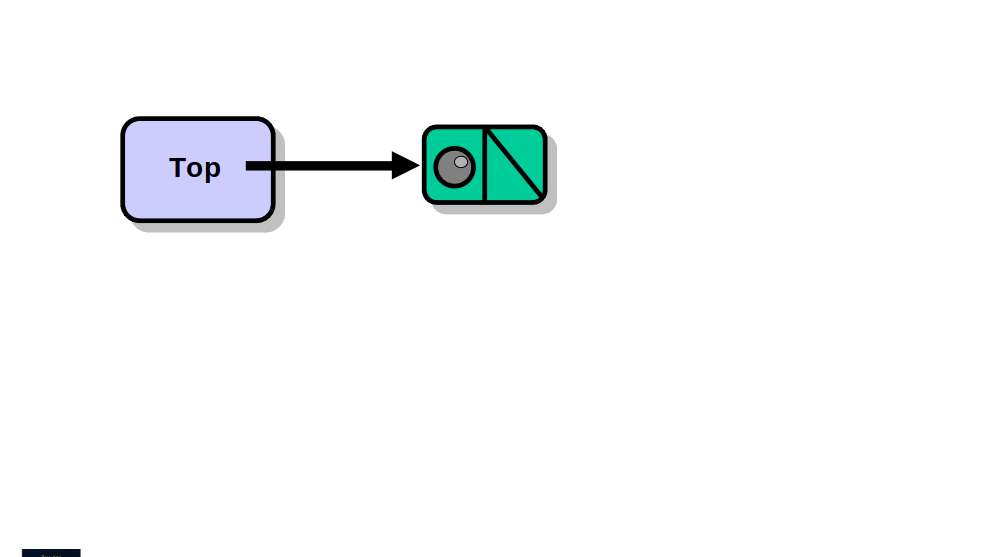
\includegraphics[width=0.5\textwidth]{./pics/stack/117.png} \end{center} }
\only<2>{ \begin{center} 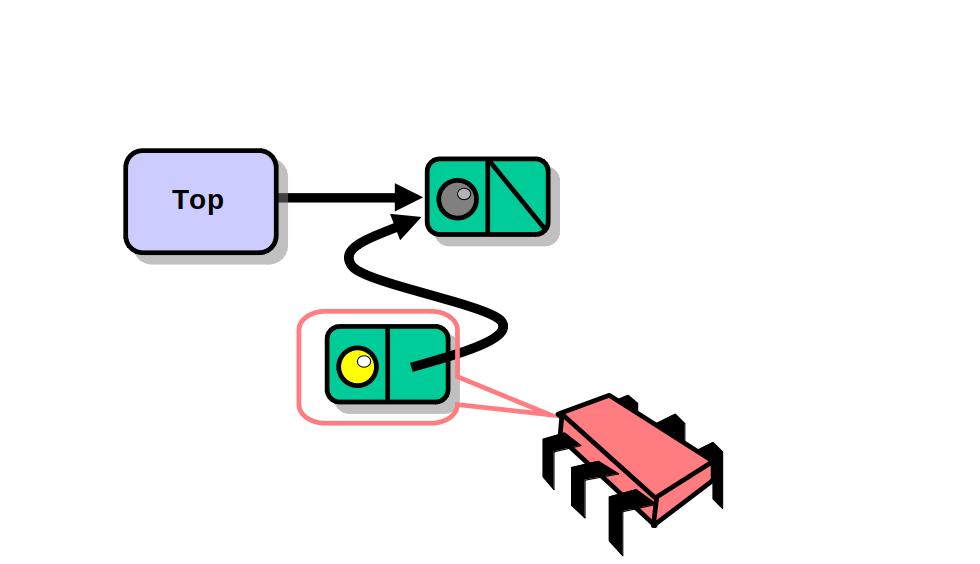
\includegraphics[width=0.5\textwidth]{./pics/stack/118.png} \end{center} }
\only<3>{ \begin{center} 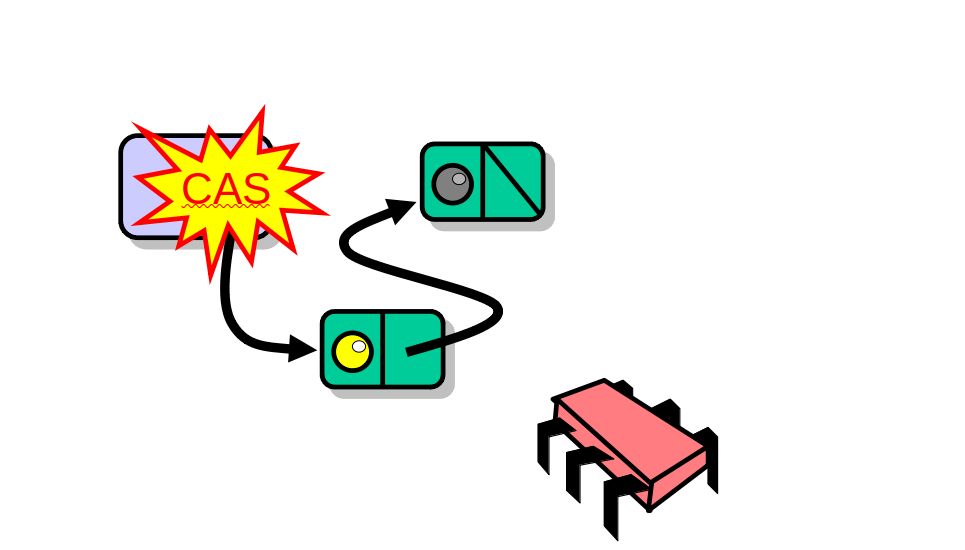
\includegraphics[width=0.5\textwidth]{./pics/stack/119.png} \end{center} }
\only<4>{ \begin{center} 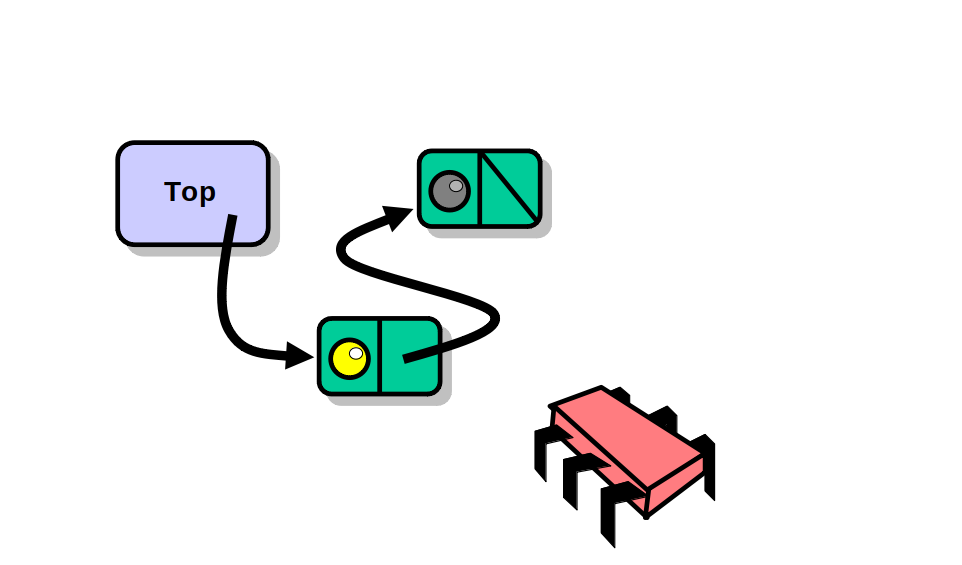
\includegraphics[width=0.5\textwidth]{./pics/stack/120.png} \end{center} }
\only<5>{ \begin{center} 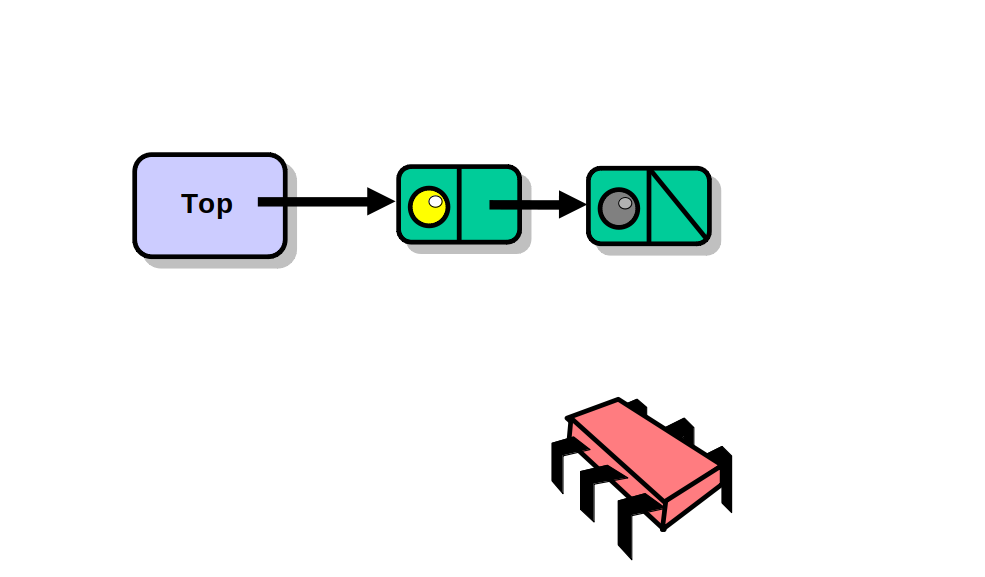
\includegraphics[width=0.5\textwidth]{./pics/stack/121.png} \end{center} }
\only<6>{ \begin{center} 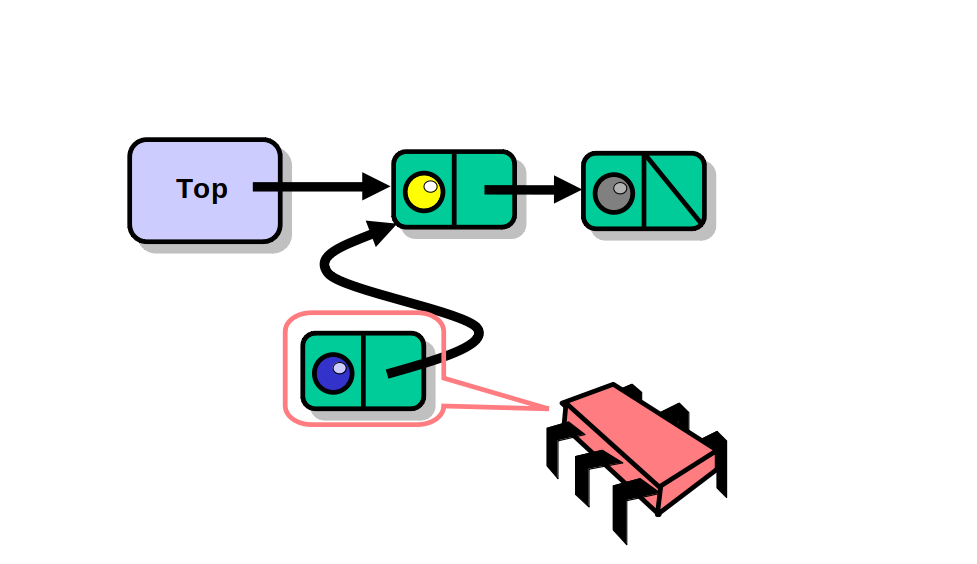
\includegraphics[width=0.5\textwidth]{./pics/stack/122.png} \end{center} }
\only<7>{ \begin{center} 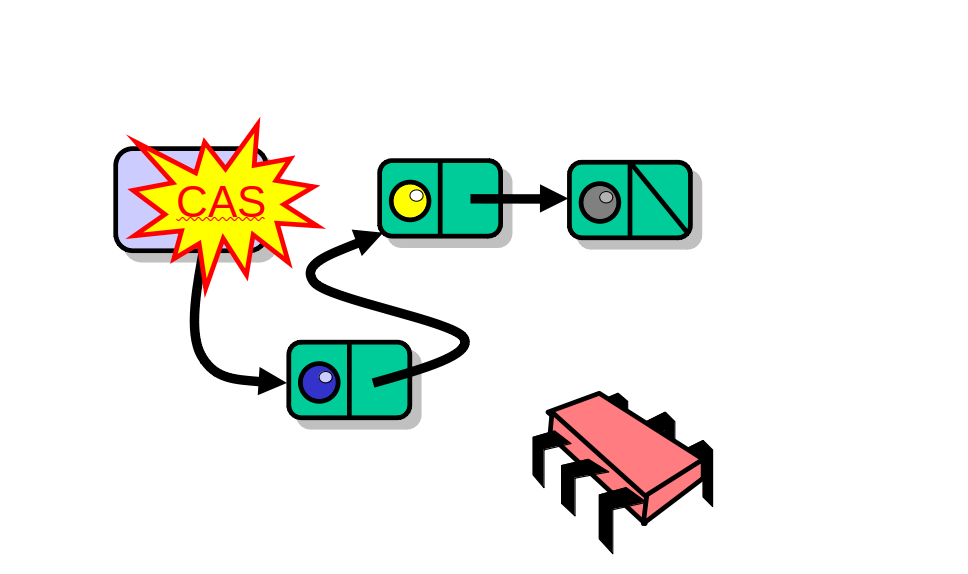
\includegraphics[width=0.5\textwidth]{./pics/stack/123.png} \end{center} }
\only<8>{ \begin{center} 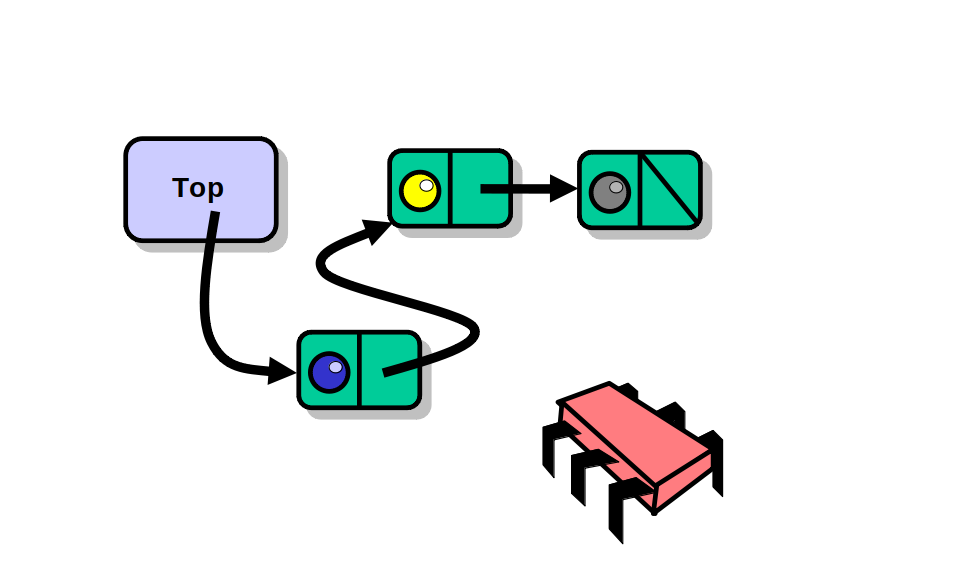
\includegraphics[width=0.5\textwidth]{./pics/stack/124.png} \end{center} }
\end{frame}


\begin{frame}{Lock-free stack: pop}
\only<1>{ \begin{center} 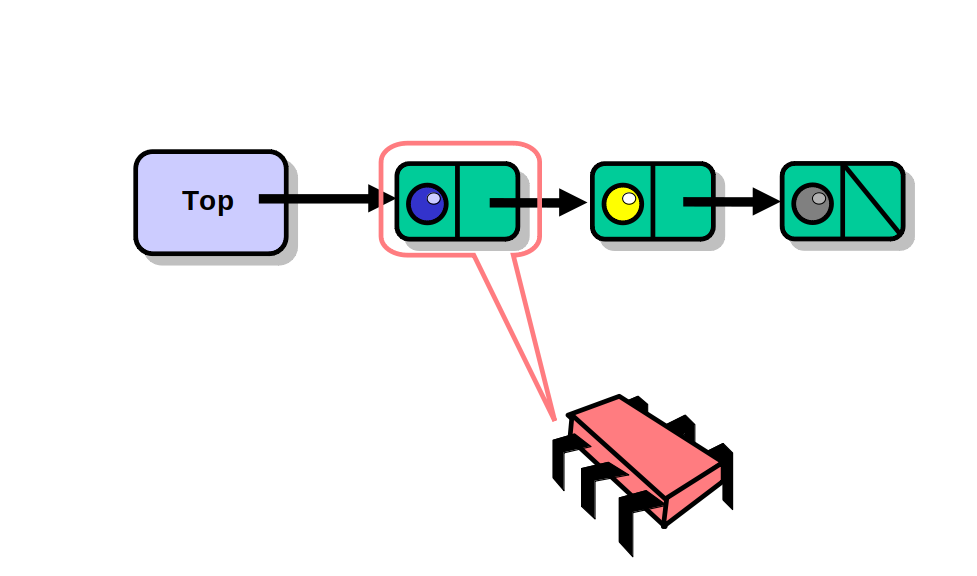
\includegraphics[width=0.5\textwidth]{./pics/stack/125.png} \end{center} }
\only<2>{ \begin{center} 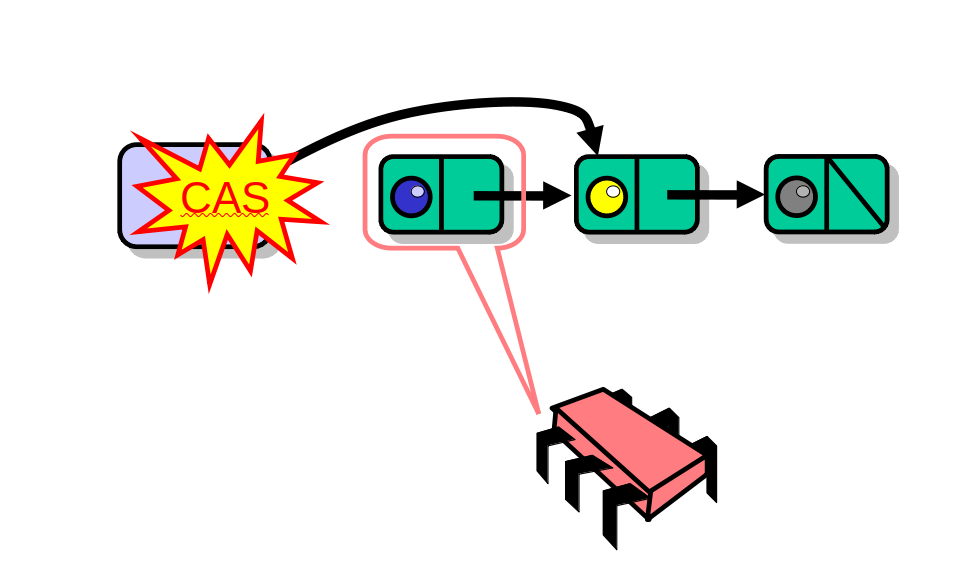
\includegraphics[width=0.5\textwidth]{./pics/stack/126.png} \end{center} }
\only<3>{ \begin{center} 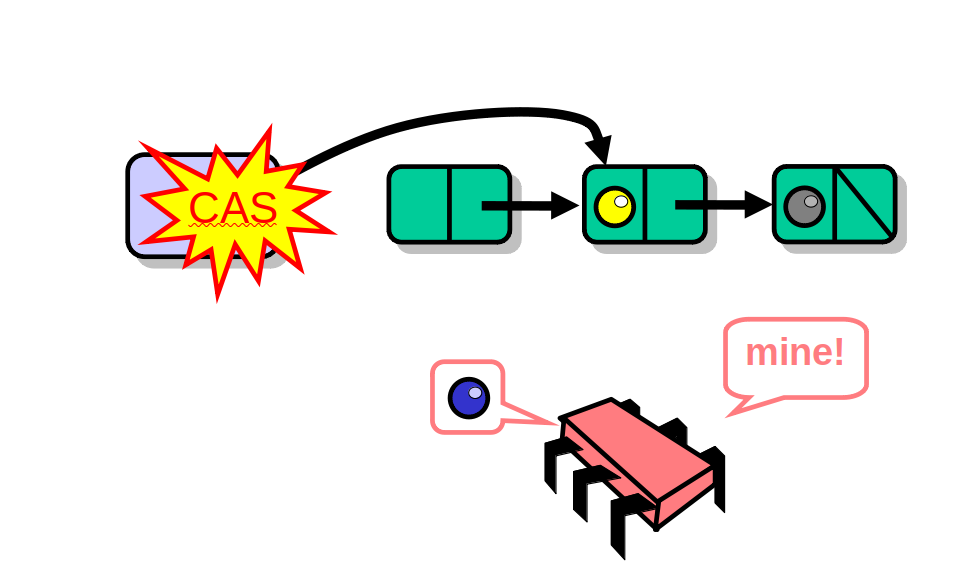
\includegraphics[width=0.5\textwidth]{./pics/stack/127.png} \end{center} }
\only<4>{ \begin{center} 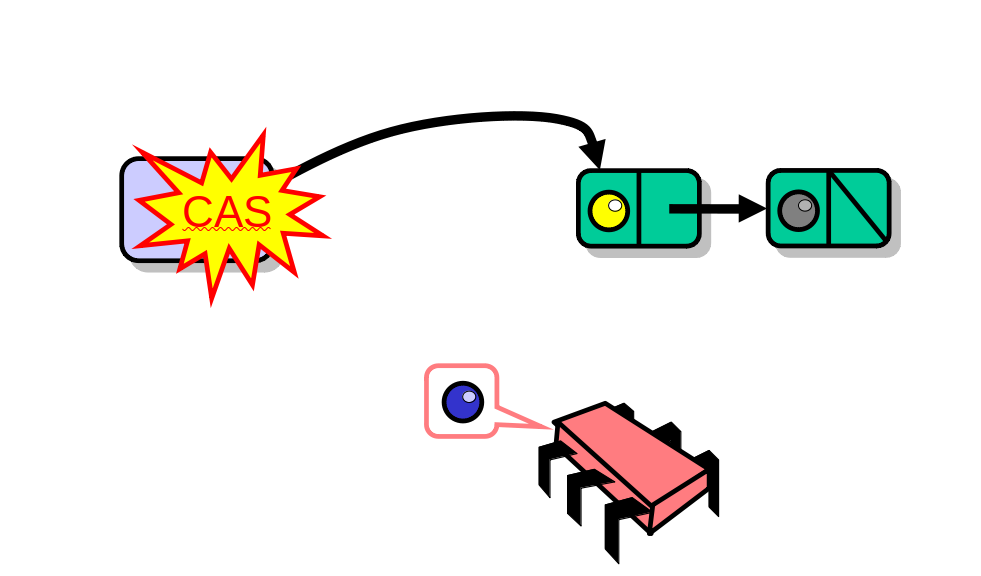
\includegraphics[width=0.5\textwidth]{./pics/stack/128.png} \end{center} }
\only<5>{ \begin{center} 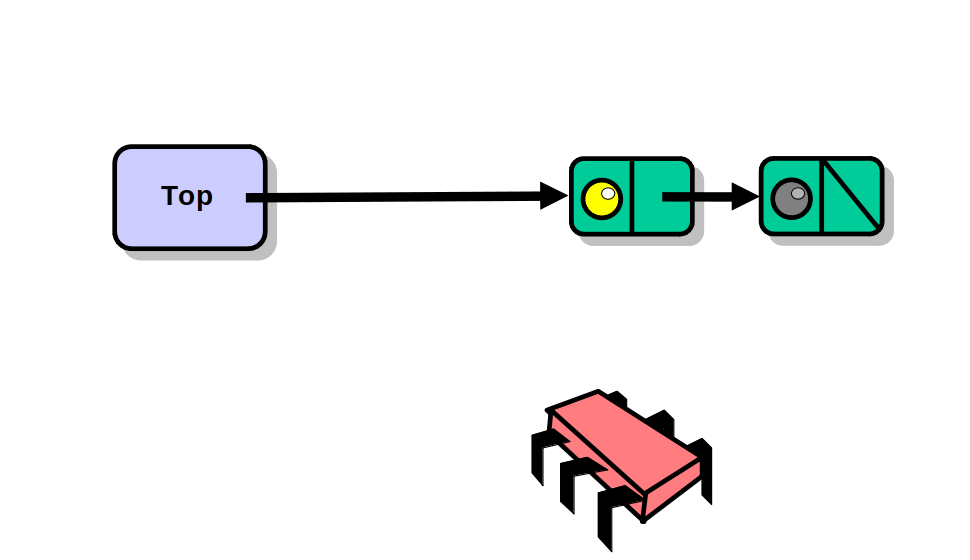
\includegraphics[width=0.5\textwidth]{./pics/stack/129.png} \end{center} }
\end{frame}


\begin{frame}[fragile]{Lock-free stack}
\begin{minted}{java}
public class LockFreeStack {
  private AtomicReference top = new AtomicReference(null); 
  public boolean tryPush(Node node){
    Node oldTop = top.get();    
    node.next = oldTop;
    return top.compareAndSet(oldTop, node);
  }
  public void push(T value) {
    Node node = new Node(value); 
    while (true) {
      if (tryPush(node)) return;
      backoff.backoff();
  }}
\end{minted}

\pause
\begin{itemize}
  \item Wait-free, lock-free or obstruction-free?
\end{itemize}

\end{frame}

\begin{frame}[fragile]{Lock-free stack: summary}

\begin{itemize}
  \item Your first non-trivial and useful lock-free algorithm based on RMW
  \item Elegant
  \item Easy to reason about
  \item Easy to define linearization points
\end{itemize}

\pause

But not perfect?

\end{frame}

\begin{frame}[fragile]{Node pooling}

\begin{minted}{java}
public class LockFreeStack {
  private AtomicReference top = new AtomicReference(null); 
  public boolean tryPush(Node node){
    Node oldTop = top.get();    
    node.next = oldTop;
    return top.compareAndSet(oldTop, node);
  }
  public void push(T value) {
    Node node = new Node(value); // Yikes!
    while (true) {
      if (tryPush(node)) return;
      backoff.backoff();
  }}
\end{minted}

\end{frame}


\begin{frame}[fragile,noframenumbering]{Node pooling}

\begin{minted}{java}
public class LockFreeStack {
  private AtomicReference top = new AtomicReference(null); 
  public boolean tryPush(Node node){
    Node oldTop = top.get();    
    node.next = oldTop;
    return top.compareAndSet(oldTop, node);
  }
  public void push(T value) {
    Node node = ThreadLocalNodePool.get(); // successful `pop` 
    //                                        will populate this cache
    node.value = value;
    while (true) {
      if (tryPush(node)) return;
      backoff.backoff();
  }}
\end{minted}
\end{frame}


\begin{frame}[t,fragile]{ABA problem}
\begin{center}
\begin{tikzpicture}[node distance=2cm,on grid,every state/.style={thick}]
  \node[state]  (top)              {$top$};
  \node[state,draw=none]  (E) [above=of A] {};
  \node[state]  (A) [right=of main] {$A$};
  \node[state]  (B) [right=of A]    {$B$};
  \node[state]  (N) [right=of B]    {$null$};

  \path[->] (top) edge  node   {} (A)
            (A) edge  node   {} (B)
            (B) edge  node   {} (N);
\end{tikzpicture}
\end{center} 

\begin{tabular}{p{5cm}p{5cm}}
Thread 1 & Thread 2 \\
\end{tabular}
\end{frame}



\begin{frame}[t,fragile,noframenumbering]{ABA problem}
\begin{center}
\begin{tikzpicture}[node distance=2cm,on grid,every state/.style={thick}]
  \node[state]  (top)              {$top$};
  \node[state,draw=none]  (E) [above=of A] {};
  \node[state]  (A) [right=of main] {$A$};
  \node[state]  (B) [right=of A]    {$B$};
  \node[state]  (N) [right=of B]    {$null$};

  \path[->] (top) edge  node   {} (A)
            (A) edge  node   {} (B)
            (B) edge  node   {} (N);
\end{tikzpicture}
\end{center} 

\begin{tabular}{p{5cm}p{5cm}}
Thread 1 & Thread 2 \\
\textbf{Start \texttt{pop()}} (\texttt{top.CAS(A, B)}) &
\end{tabular}

\end{frame}



\begin{frame}[t,fragile,noframenumbering]{ABA problem}
\begin{center}
\begin{tikzpicture}[node distance=2cm,on grid,every state/.style={thick}]
  \node[state]  (top)               {$top$};
  \node[state,draw=none]  (E) [right=of main] {};
  \node[state]  (A) [above=of E]    {$A$};
  \node[state]  (B) [right=of E]    {$B$};
  \node[state]  (N) [right=of B]    {$null$};

  \path[->] (top) edge node {} (B)
            (A) edge  node   {} (B)
            (B) edge  node   {} (N);
\end{tikzpicture}
\end{center} 

\begin{tabular}{p{5cm}p{5cm}}
Thread 1 & Thread 2 \\
Start \texttt{pop()} (\texttt{top.CAS(A, B)}) & \\
                     &  \texttt{A = pop()} \\
\end{tabular}
\end{frame}


\begin{frame}[t,fragile,noframenumbering]{ABA problem}
\begin{center}
\begin{tikzpicture}[node distance=2cm,on grid,every state/.style={thick}]
  \node[state]  (top)               {$top$};
  \node[state,draw=none]  (E) [right=of main] {};
  \node[state]  (A) [above=of E]    {$A$};
  \node[state]  (B) [right=of E]    {$B$};
  \node[state]  (N) [right=of B]    {$null$};

  \path[->] (top) edge node {} (B)
            (A) edge  node   {} (B)
            (B) edge  node   {} (N);
\end{tikzpicture}
\end{center} 

\begin{tabular}{p{5cm}p{5cm}}
Thread 1 & Thread 2 \\
Start \texttt{pop()} (\texttt{top.CAS(A, B)}) & \\
                     &  \texttt{A = pop()} \\
                     &  \texttt{reclaim(A)} \\
\end{tabular}
\end{frame}

\begin{frame}[t,fragile,noframenumbering]{ABA problem}
\begin{center}
\begin{tikzpicture}[node distance=2cm,on grid,every state/.style={thick}]
  \node[state]  (top)               {$top$};
  \node[state]  (C) [right=of main] {$C$};
  \node[state]  (A) [above=of E]    {$A$};
  \node[state]  (B) [right=of E]    {$B$};
  \node[state]  (N) [right=of B]    {$null$};

  \path[->] (top) edge node {} (C)
            (C) edge  node   {} (B)
            (A) edge  node   {} (B)
            (B) edge  node   {} (N);
\end{tikzpicture}
\end{center} 

\begin{tabular}{p{5cm}p{5cm}}
Thread 1 & Thread 2 \\
Start \texttt{pop()} (\texttt{top.CAS(A, B)}) & \\
                     &  \texttt{A = pop()} \\
                     &  \texttt{reclaim(A)} \\
                     &  \texttt{push(C)} \\                     
\end{tabular}
\end{frame}

\begin{frame}[t,fragile,noframenumbering]{ABA problem}
\begin{center}
\begin{tikzpicture}[node distance=2cm,on grid,every state/.style={thick}]
  \node[state]  (top)               {$top$};
  \node[state]  (C) [right=of main] {$C$};
  \node[state]  (A) [above=of E]    {$A$};
  \node[state]  (B) [right=of E]    {$B$};
  \node[state]  (N) [right=of B]    {$null$};

  \path[->] (top) edge node {} (C)
            (C) edge  node   {} (B)
            (A) edge  node   {} (B)
            (B) edge  node   {} (N);
\end{tikzpicture}
\end{center} 

\begin{tabular}{p{5cm}p{5cm}}
Thread 1 & Thread 2 \\
Start \texttt{pop()} (\texttt{top.CAS(A, B)}) & \\
                     &  \texttt{A = pop()} \\
                     &  \texttt{reclaim(A)} \\
                     &  \texttt{push(C)} \\                     
                     &  \texttt{push(A')} \\                                          
\end{tabular}
\end{frame}

\begin{frame}[t,fragile,noframenumbering]{ABA problem}
\begin{center}
\begin{tikzpicture}[node distance=2cm,on grid,every state/.style={thick}]
  \node[state]  (top)               {$top$};
  \node[state]  (C) [right=of main] {$C$};
  \node[state]  (A) [above=of E]    {$A$};
  \node[state]  (B) [right=of E]    {$B$};
  \node[state]  (N) [right=of B]    {$null$};

  \path[->] (top) edge node {} (A)
            (C) edge  node   {} (B)
            (A) edge  node   {} (C)
            (B) edge  node   {} (N);
\end{tikzpicture}
\end{center} 

\begin{tabular}{p{5cm}p{5cm}}
Thread 1 & Thread 2 \\
Start \texttt{pop()} (\texttt{top.CAS(A, B)}) & \\
                     &  \texttt{A = pop()} \\
                     &  \texttt{reclaim(A)} \\
                     &  \texttt{push(C)} \\                     
                     &  \texttt{push(A')} \\                                          
\end{tabular}
\end{frame}

\begin{frame}[t,fragile,noframenumbering]{ABA problem}
\begin{center}
\begin{tikzpicture}[node distance=2cm,on grid,every state/.style={thick}]
  \node[state]  (top)               {$top$};
  \node[state]  (C) [right=of main] {$C$};
  \node[state]  (A) [above=of E]    {$A$};
  \node[state]  (B) [right=of E]    {$B$};
  \node[state]  (N) [right=of B]    {$null$};

  \path[->] (top) [bend right, below] edge  node {} (B);
  \path[->]
            (C) edge  node   {} (B)
            (A) edge  node   {} (C)
            (B) edge  node   {} (N);
\end{tikzpicture}
\end{center} 

\begin{tabular}{p{5cm}p{5cm}}
Thread 1 & Thread 2 \\
Start \texttt{pop()} (\texttt{top.CAS(A, B)}) & \\
Finish \texttt{pop()} &  \texttt{A = pop()} \\
                     &  \texttt{reclaim(A)} \\
                     &  \texttt{push(C)} \\                     
                     &  \texttt{push(A')} \\                                          
\end{tabular}
\end{frame}



\begin{frame}{ABA problem}

ABA problem is always a headache in non-GC languages. 

It still happens in managed languages, be aware.

Advanced algorithms you could or could not use:
\begin{itemize}
 \item \texttt{AtomicStampedReference}\footnote{\tiny\url{https://docs.oracle.com/en/java/javase/11/docs/api/java.base/java/util/concurrent/atomic/AtomicStampedReference.html}}
 \item immortal memory
 \item RCU
 \item reference counting
 \item other variation of GC
 \item hazard pointers
 \item ...
\end{itemize}

\end{frame}


\section{Summary}

\begin{frame}{Summary}

Read-Modify-Write atomic operations
\begin{itemize}
 \item \texttt{getAndSet}, \texttt{getAndAdd} -- consensus number \textbf{2}
 \item \texttt{compareAndSet}, \texttt{compareAndExchange} -- consensus number $\infty$
\end{itemize}

Spin locks
\begin{itemize}
  \item Test-and-set
  \item Test-and-test-and-set
  \item Exponential Backoff
\end{itemize}

Memory hierarchy
\begin{itemize}
  \item Multi-level caching
  \item Cache coherence via replication and message passing
  \item Invalidation storm  
\end{itemize}

Lock-free stack and ABA for pooling.

\end{frame}

\begin{frame}{Summary: homework}

\begin{homeworkmail}{Task~\taskReentrantTAS}{
    Replace \texttt{AtomicBoolean} with \texttt{AtomicReference(Thread.cuurentThread)} and make TAS lock reentrant. Provide at least 3 tests written in JCStress.
}
\end{homeworkmail}

\begin{homeworkmail}{Task~\taskSpinMeasure}{
    Measure performance of \texttt{TASLock}, \texttt{TATASLock}, \texttt{ExpBackoffLock} on
    \begin{itemize}
      \item 1, 2, 3, 4, 5, 6, 7, 8, 16, 32 concurrent threads
      \item With small critical section (increment)
      \item With moderate critical section (compute n-th fibonacci number recursively)
    \end{itemize}
    using JMH or JCStress, plot resulting figures (with error bars!), explain gathered data.
}
\end{homeworkmail}

\end{frame}


% \begin{frame}{Ticket lock}
% 
% now we need fairness and trivial atomic impl
% 
% conclusion: not good but we implemented it with fetch-and-inc (consensu=2), not with cAS (consensu=inf)
% 
% So now you know the IDEAS:
% peterson lock (2 threads, 2 regs)
% FIlter lock (N thread, N regs)
% Ticket lock (inf thread, f-and-add)
% TATAS lock (inf thread, CAS)
% 
% TODO: lecTODO will add queue-based lock ieas to your arsenal
% 
% \end{frame}


% 
% \begin{frame}{Lock free data structures}
% 
% we have atomics, may try to prifduce something more interesting in terms of progress guarantes (wait free , lock free,  obstruct free )
% 
% even cocncurrent sigle linked lists are CHAPTERS of dedicated books, imagine literature on
% - diuble-link lists
% - queue
% - hash tables
% - sets
% - trees
% etc
% 
% To SIMPLIFY we will use GC-assisted language (no mem corrutp, no use after free, no object identity ABA)
% 
% \end{frame}
% 
% 
% \begin{frame}{Queus}
% taxonomy
  % MPSC MPPC ...
  % wait-free lock free
  % bounded unbounded
% 
% 
% SEE 1000cores vjukov
% 
% we will discuss few samples
% 
% \end{frame}
% 
% \begin{frame}{wait-free SPSC}
% 
% bounded?
% 
% \end{frame}
% 
% 
% \begin{frame}{unbound lock free MPMC}
% 
% \end{frame}
% 
% 
% \begin{frame}{unbound lock free MPMC}
% adding lock-free free list for memory management
% 
% and woo hoo cerash
% 
% 
% CONCLUSION: you are not ready for concurrency in unmanaged languages
% at all
% 
% adding stamps/markers, wrapping stamps etc
% 
% Further reading: marked pointers, colored pinters, hazard pointers
% 
% \end{frame}
% 
% 
% \begin{frame}{unexplained real life phenomena}
% 
% Cahe contetntion and mem bus traffix 
 % false sharing
 % real sharing
% 
% visibility issues
% - variations of atomics (seq-cst, relazed)
% - variation of filed (USUAL, FINAL, VOLATILE)
% 
% We need to go deeper and talk a few words on processor level (highest level of abstraction, by the way)
% 
% \end{frame}


\end{document}
